\documentclass[a4paper]{cas-sc}

\usepackage[authoryear]{natbib}
\usepackage{setspace}
% Author macros
\def\tsc#1{\csdef{#1}{\textsc{\lowercase{#1}}\xspace}}
\tsc{WGM}
\tsc{QE}

\usepackage{amssymb}
\usepackage{amsmath,amsfonts}
\usepackage{caption}
\captionsetup[figure]{
  name={Fig.},
  labelsep=colon,
  font={rm,small},
  labelfont=bf,
  justification=raggedright,
  singlelinecheck=off,
  skip=4pt,
}
\setlength{\textfloatsep}{8pt plus 2pt minus 2pt}
\setlength{\floatsep}{8pt plus 2pt minus 2pt}
\setlength{\intextsep}{8pt plus 2pt minus 2pt}
\renewcommand{\topfraction}{0.95}
\renewcommand{\bottomfraction}{0.95}
\renewcommand{\textfraction}{0.05}
\renewcommand{\floatpagefraction}{0.8}
% Patch cas-common.sty: replace \sffamily with \rmfamily in caption functions to match body text
\ExplSyntaxOn
\cs_set:Npn \__make_tbl_caption:nn #1#2
{
  \l_tbl_align_tl
  \skip_vertical:N \l_tbl_abovecap_skip
  {\parbox{\dimexpr(\l_tbl_width_dim)}
    {\setstretch{1}\rightskip=0pt\rmfamily\small\textbf{\color{scolor}#1}\par#2\par\vskip2pt}}
  \skip_vertical:N \l_tbl_belowcap_skip
}
\cs_set:Npn \__make_fig_caption:nn #1#2
{
  \l_fig_align_tl
  \skip_vertical:N \l_fig_abovecap_skip
  \setbox\cascaptionbox=\hbox{%
    \setstretch{1}\rmfamily\small\textbf{\color{scolor}#1:}~#2}
  \ifdim\the\wd\cascaptionbox<\dim_use:N \l_fig_width_dim\relax
    \parbox{\l_fig_width_dim}
      {\setstretch{1}\raggedright\unskip\ignorespaces\rmfamily\small\textbf{\color{scolor}#1:}~#2\par}
  \else
    \parbox{\l_fig_width_dim}
      {\setstretch{1}\raggedright\unskip\ignorespaces\rmfamily\small\textbf{\color{scolor}#1:}~#2\par}
  \fi
  \skip_vertical:N \l_fig_belowcap_skip
}
% Patch cas-common.sty: suppress ORCID line and customize first-page footer text
\RenewDocumentCommand \printorcid { } { }
\cs_set:Npn \__first_footerline:
{
  \group_begin:
  \scriptsize
  \sffamily
  \ifnum\theblind>0\relax
  \else
    \__short_authors: :~
  \fi
  { \rmfamily \itshape Preprint~submitted~to~Energy }
  \group_end:
}
\ExplSyntaxOff
\usepackage[linesnumbered,ruled]{algorithm2e}
\usepackage{array}
\usepackage{textcomp}
\usepackage{stfloats}
\usepackage{float}
\usepackage{placeins}
\usepackage{url}
\usepackage{verbatim}
\usepackage{graphicx}
\usepackage{epstopdf}
\epstopdfsetup{outdir=./build/}
\graphicspath{{./}{./build/}}
\usepackage{multirow}
\usepackage{mathrsfs}
\usepackage{amsthm}
\newtheorem{myDef}{Definition}
\newtheorem{myTheo}{Theorem}
\newtheorem{mypro}{Proposition}
\newtheorem{myex}{Example}
\usepackage{booktabs}
\usepackage{threeparttable}
\usepackage{etoolbox}
\captionsetup[table]{
  labelsep=newline,
  singlelinecheck=false,
  skip=4pt,
}
\AtBeginEnvironment{table}{\rmfamily\normalsize}
\AtBeginEnvironment{table*}{\rmfamily\normalsize}
\AtBeginEnvironment{tabular}{\rmfamily\normalsize}
\usepackage{hyperref}
\hypersetup{%hypertex=true,
            colorlinks=true,
            linkcolor=blue,
            anchorcolor=blue,
            citecolor=blue}
\newtheorem{remark}{Remark}
\renewcommand{\qedsymbol}{}
\renewcommand{\theenumi}{\arabic{enumi}}
\renewcommand{\labelenumi}{(\theenumi)}
\setlength{\bibsep}{0pt}
\AtBeginEnvironment{thebibliography}{\singlespacing\scriptsize\setlength{\parskip}{0pt}\setlength{\itemsep}{0pt}}
% Keep abstract in main.tex to make SyncTeX jump to the source file.
\makeatletter
\ExplSyntaxOn
\tl_new:N \g__cas_abs_tl

\RenewDocumentEnvironment { abstract } { o +b }
{
  \IfNoValueTF { #1 } { }
   { \tex_gdef:D \abstracttitle { #1 } }
  \tl_gset:Nn \g__cas_abs_tl { #2 }
}
{ }

\AtBeginDocument{\onehalfspacing}

\RenewDocumentCommand \MaketitleBox { O{} }
{
  \tl_if_blank:nTF { #1 } { }
  { \keys_set:nn { stm / mktitle } { #1 } }
  \processbreakafter
  \singlespacing
  \group_begin:
  \@title
  \group_end:
  %
  \bool_if:NTF \g_stm_blind_bool
  { \vspace* { 10 mm } }
  {
    \group_begin:
    \normalsize \stmauthors \par
    \stmcollab \par
    \footnotesize \itshape \stmaddress \par
    \group_end:
    \bool_if:NTF \g_stm_breakafter_auaff_bool
    { \newpage } { }
  }
  % \printFirstPageNotes
  %
  \dashrule{0pt}{3pt}
  \begin{Abstract}
    \noindent \ignorespaces
    \tl_use:N \g__cas_abs_tl
  \end{Abstract}
  \dashrule{6pt}{3pt}
  \bool_if:NTF \g_stm_breakafter_abstract_bool
  { \newpage } { }
  \onehalfspacing
}

\RenewDocumentCommand \LongMaketitleBox { O{} }
{
  \tl_if_blank:nTF { #1 } { }
  { \keys_set:nn { stm / mktitle } { #1 } }
  \vbox_gset:Nn \g_stm_front_box
  {
    \singlespacing
    \group_begin:
    \@title
    \group_end:
    %
    \bool_if:NTF \g_stm_blind_bool
     { \vspace* { 10 mm } }
     { \group_begin:
       \normalsize \stmauthors \par
       \stmcollab \par
       \footnotesize \itshape \stmaddress \par
       \group_end:
     }
  %
  \dashrule{0pt}{3pt}
  \begin{Abstract}
    \noindent \ignorespaces
    \tl_use:N \g__cas_abs_tl
  \end{Abstract}
  \dashrule{3pt}{3pt}
  }
  \vbox_gset:Nn \g_stm_notes_box
  {  \cs_set_eq:NN \footnotetext \__fn_text:n  \printFirstPageNotes }
   \dim_gset:Nn \g_tmpb_dim { \box_ht:N \g_stm_notes_box }
   % \iow_term:x { ...~[ht: \dim_use:N \g_tmpb_dim  ] }
   \dim_gadd:Nn \g_tmpb_dim { \box_dp:N \g_stm_notes_box }
   % \iow_term:x { ...~[ht+dp: \dim_use:N \g_tmpb_dim  ] }
   \ifbool{sc}{\dim_gadd:Nn \g_tmpb_dim { 12pt } } { }
}
\ExplSyntaxOff
\makeatother

\begin{document}
\let\WriteBookmarks\relax
\def\floatpagepagefraction{1}
\def\textpagefraction{.001}

%------------------------ Title ------------------------

\title [mode = title]{Transfer Learning Quantile Large-margin Distribution Machine for Wind Power Forecasting under Extreme Events}
\shorttitle{}

%------------------------ Authors ------------------------
\shortauthors{Junlin Chen et~al.}

\author[1]{Junlin Chen}
\credit{Methodology, Software, Writing - original draft}
\affiliation[1]{
    organization={School of Management and Engineering, Nanjing University},
    city={Nanjing},
    citysep={},
    postcode={210093},
    country={China}}

\affiliation[2]{
    organization={Department of Information Engineering and Computer Science, Feng Chia University},
    city={Taichung},
    citysep={},
    postcode={40724},
    country={China}}

\affiliation[3]{
    organization={College of Artificial Intelligence, Southwest University},
    city={Chongqing},
    citysep={},
    postcode={400715},
    country={China}}

\affiliation[4]{
    organization={Graduate School of Information, Production and Systems, Waseda University},
    city={Kitakyushu},
    citysep={},
    postcode={808-0135},
    country={Japan}}

\author[1]{Bo Wang}
\cormark[1]
\credit{Writing -- review $\&$ editing, Funding acquisition}
\cortext[cor1]{Corresponding author: Bo Wang\\
\qquad \qquad E-mail address: jlchen08@163.com (J. Chen), bowangsme@nju.edu.cn (B. Wang), zhihangyu@smail.nju.edu.cn (Z. Yu),\\
\qquad \qquad  linrenju7@163.com (R. Lin), peiclin@fcu.edu.tw (P. Lin), lbzhang@swu.edu.cn (L. Zhang), junzo.watada.ips@gmail.com (J. Watada)
}

\author[1]{Zhihang Yu}
\credit{Formal analysis, Software}

\author[1]{Renju Lin}
\credit{Software}

\author[2]{Pei-chun Lin}
\credit{Validation, Supervision}

\author[3]{Libo Zhang}
\credit{Funding acquisition}

\author[4]{Junzo Watada}
\credit{Validation, Supervision}

%------------------------ Abstract ------------------------
\begin{abstract}
Accurate wind power forecasting under extreme events is critical for grid stability and renewable energy integration, yet remains a formidable challenge due to severe data scarcity and substantial distribution shifts between normal and extreme-event operating regimes. While kernel-based methods, particularly support vector regression and Large-margin Distribution Machine-based Regression (LDMR), have demonstrated strong performance in various regression tasks due to their theoretical guarantees and robustness on limited data, their application to extreme-event forecasting faces critical limitations: the i.i.d. assumption underlying standard kernel methods is fundamentally violated under cross-domain scenarios, and the symmetric variance minimization in LDMR implicitly encourages symmetric error distributions, which conflicts with the asymmetric nature of quantile-based interval prediction required for uncertainty quantification. To extend kernel-based regression to extreme-event forecasting, we propose Transfer Learning Quantile Large-margin Distribution Machine for Regression (TL-QLDMR), which addresses these challenges through three synergistic innovations: (i) an asymmetric variance regularizer that preserves LDMR's distributional robustness while accommodating quantile-specific error asymmetry, (ii) a supervised transfer learning framework integrating maximum mean discrepancy for feature alignment and weighted pinball loss for label adaptation, enabling effective knowledge transfer from abundant normal-domain data to scarce extreme-event samples, and (iii) a scalable Nystr\"{o}m-SGD solver reducing complexity from $O(N^3)$ to $O(T \cdot N \cdot m)$. Comprehensive experiments on six wind farms demonstrate that TL-QLDMR achieves competitive performance in both deterministic and probabilistic forecasting in the extreme-event domain, with superior reliability-sharpness trade-off and practical scalability, making it suitable for real-time applications where interpretability and theoretical guarantees are prioritized.
\end{abstract}


%------------------------ Keywords ------------------------
\begin{keywords}
Wind power forecasting\\
Large-margin distribution machine\\
Quantile regression\\
Transfer learning\\
Extreme events
\end{keywords}

\maketitle

%% main text
%------------------------ Introduction ------------------------
\section{Introduction}

The global transition toward renewable energy has positioned wind power as a cornerstone of sustainable electricity generation. However, the inherent intermittency and volatility of wind resources pose significant challenges to power-system reliability, reserve allocation, and dispatch efficiency \citep{yuan2023conditional}. Accurate wind power forecasting is therefore critical for reducing balancing costs, supporting storage planning, and enabling secure grid integration \citep{yan2025economic, wang2025ensemble}. While substantial progress has been achieved in short-term forecasting under normal meteorological conditions, prediction performance can degrade significantly during extreme events, particularly those associated with typhoons, cold waves, or heat waves, when wind power fluctuations are most severe and energy-system operations are under the greatest stress \citep{wang2024scarcity, liu2024extreme, liu2025diffusion}.
Extreme events present a dual challenge for data-driven forecasting models. First, such events are inherently rare, resulting in severe data scarcity: extreme-condition samples typically constitute only a small fraction of historical records \citep{s41597-022-01696-6, wang2024scarcity}. Second, the dynamics under extreme-event conditions differ fundamentally from normal operating regimes, inducing substantial distribution shifts in both feature space (e.g., wind speed, temperature) and label space. 

Among the diverse landscape of forecasting methodologies, kernel-based approaches, particularly Support Vector Regression (SVR) and its variants, have been extensively applied to wind power forecasting and have demonstrated competitive performance under normal-operating conditions \citep{wang2019review, zeng2011svmwind, li2021cuckoo, yuan2022jellyfish}. These kernel methods offer several distinctive advantages over black-box deep learning models: strong generalization guarantees, effective handling of high-dimensional feature spaces through the kernel trick, convex optimization formulations, and robust performance on small-to-medium-sized datasets. Recent studies have further enriched kernel regression through robust support vector machine (SVM) formulations \citep{trafalis2006robust}, bounded-loss regression \citep{fu2023bounded}, and multiple-kernel learning with compound regularization \citep{jiang2021rlmkl}, reinforcing the continuing relevance of robustness-oriented kernel learning for forecast tasks involving noisy and heterogeneous data.

Despite these strengths, existing kernel-based wind power forecasting studies predominantly focus on normal-operating conditions with deterministic point prediction objectives. To address the need for uncertainty quantification, Support Vector Quantile Regression (SVQR) extends SVR by replacing the symmetric $\epsilon$-loss with the asymmetric pinball loss, enabling estimation of conditional quantiles for prediction intervals \citep{ye2025nfs, tsvqr2023}. Recent studies have further pushed the field toward joint deterministic-probabilistic optimization, diffusion-based uncertainty modeling, and more expressive spatio-temporal forecasting architectures \citep{wang2025ensemble, liu2025diffusion, zhang2026gwsstnet}. Despite these methodological advances, the application of kernel-based methods to extreme-event forecasting remains largely unexplored, presenting both challenges and opportunities for methodological extension.

At the methodological level, a fundamental limitation shared by both SVR and SVQR is that they optimize only the minimum margin while ignoring the statistical distribution of margins across the entire dataset. To overcome this limitation, the Large-margin Distribution Machine-based Regression (LDMR) paradigm was introduced, which explicitly optimizes both the mean and variance of the margin distribution \citep{zhang2019optimal, gupta2021least}. By concentrating prediction errors tightly around zero, LDMR achieves superior generalization compared to classical SVR on a wide range of regression tasks \citep{gupta2021least, hazarika2023mode}. However, LDMR has not been systematically applied to wind power forecasting, particularly under extreme-event conditions where both distributional robustness and probabilistic interval prediction are required. These characteristics make it a promising candidate for extension to forecasting in the extreme-event domain.

Against this backdrop, extending kernel-based methods from the normal-operating domain to the extreme-event domain introduces three critical challenges. First, the i.i.d. assumption is systematically violated when transferring knowledge from normal (source domain) to extreme-event (target domain) conditions. Recent wind-power studies have explored transfer learning and domain adaptation \citep{yin2021serioparallel, wang2024scarcity, dong2023mdan}; however, their principled integration with kernel-based regression remains open. Second, there exists a fundamental theoretical tension between LDMR's variance minimization, which implicitly encourages symmetric error distributions, and quantile regression at level $\tau \neq 0.5$, which requires inherently asymmetric residual distributions. Reconciling distributional robustness and quantile-specific asymmetry requires a principled modification of the LDMR framework. Third, existing transfer learning approaches for wind power forecasting predominantly adopt unsupervised adaptation strategies that underutilize scarce target-domain labels \citep{yin2021serioparallel, wang2024scarcity, dong2023mdan}. A more effective framework should leverage both feature-space alignment and label-space supervision, strategically weighting target samples to guide model adaptation.

To address these challenges, Transfer Learning Quantile Large-margin Distribution Machine for Regression (TL-QLDMR) is proposed as a principled extension of the classical LDMR paradigm for cross-domain probabilistic wind power prediction. The framework introduces three synergistic innovations. First, a novel asymmetric variance regularization mechanism reconciles the tension between distributional robustness and quantile estimation, compressing overall error dispersion while preserving the requisite skewness for accurate quantile prediction. Second, a supervised transfer learning framework integrates maximum mean discrepancy (MMD) minimization for feature-space alignment in a reproducing kernel Hilbert space (RKHS) with a weighted pinball loss mechanism that assigns substantially higher weights to scarce target-domain samples, enabling dual-space adaptation that addresses the label-neglect problem in existing unsupervised methods. Third, a scalable Nystr\"{o}m stochastic gradient descent (Nystr\"{o}m-SGD) algorithm reduces computational complexity from $O(N^3)$ to $O(T \cdot N \cdot m)$, enabling practical deployment on large-scale datasets. The main contributions of this paper are summarized as follows:

\begin{itemize}
    \item A unified TL-QLDMR framework is developed for wind power forecasting under extreme events, so that probabilistic forecasting, large-margin distribution learning, and supervised transfer adaptation are integrated into a single kernel-based objective.
    \item An asymmetric variance regularization term is designed for quantile learning, which preserves the skewed residual structure required by quantile regression while retaining the robustness advantage of the original LDMR idea.
    \item A dual-space transfer mechanism is introduced by combining MMD-based feature alignment with target-weighted pinball loss, enabling the model to exploit abundant normal-domain samples while emphasizing scarce extreme-event labels.
    \item A scalable Nystr\"{o}m-SGD solver is derived to reduce the computational burden of kernel optimization and make the proposed method applicable to large-scale supervisory control and data acquisition (SCADA) data.
    \item Extensive experiments on six wind farms verify the effectiveness of the proposed method in deterministic prediction, interval forecasting, ablation comparison, and scalability evaluation under extreme-event settings.
\end{itemize}


The remainder of this paper is organized as follows. Section~\ref{rel} reviews the theoretical foundations of LDMR and transfer learning with MMD, establishing the building blocks for our method. Section~\ref{novel} presents the TL-QLDMR formulation, including the asymmetric variance regularizer, supervised transfer framework, and scalable optimization algorithm. Section~\ref{Experiments} describes the dataset, experimental setup, and comprehensive evaluation results across deterministic prediction, probabilistic interval forecasting, ablation studies, and computational efficiency analysis. Finally, Section~\ref{conclusion} concludes the paper and discusses future research directions.

%------------------------ Related work ------------------------

\section{Related Work}\label{rel}
This section briefly reviews the theoretical foundations related to the proposed method, including LDMR and transfer learning with MMD.

\subsection{LDMR}
While SVR and SVQR focus on maximizing the minimum margin, they largely ignore the statistical distribution of the margin over the entire dataset. LDMR was proposed to improve generalization by explicitly optimizing the distribution of the margins.
From early large-margin distribution formulations to least-squares and mode-seeking variants, LDMR has evolved into a practical framework for robust learning under noisy conditions \citep{zhang2014large, zhang2019optimal, gupta2021least, hazarika2023mode}.

The key idea of LDMR is to not only maximize the margin of the support vectors but also to minimize the variance of the error distribution for all samples. A typical LDMR formulation for regression integrates two additional statistical regularization terms into the objective function
\begin{equation}
\label{eq:ldmr_concept}
\min_{\boldsymbol{w}, b} \frac{1}{2} \|\boldsymbol{w}\|^2 + \lambda_1 \text{Var}(\text{Residuals}) + \lambda_2 \text{Mean}(\text{Residuals}) + C \sum_{i=1}^{n} L(y_i, f(\boldsymbol{x}_i)),
\end{equation}
by constraining the variance, LDMR forces the prediction errors to be clustered tightly around zero, leading to a more compact and robust hypothesis space. However, this variance minimization implicitly encourages symmetric error distributions. Our work extends this concept by introducing an asymmetric variance regularization mechanism suitable for quantile regression, which preserves the distributional robustness of LDMR while accommodating the inherent asymmetry required for accurate quantile estimation.

\subsection{Transfer Learning and MMD}
Standard machine learning models operate under the assumption that training (source) and testing (target) data are drawn from the same probability distribution. When this assumption is violated, such as in wind power forecasting across different operating regimes, the model performance degrades significantly. Transfer learning aims to transfer knowledge from a label-rich source domain to a target domain with different but related distributions.
MMD-based adaptation has been widely used in transfer scenarios because it provides a non-parametric discrepancy measure in RKHS and integrates naturally with kernelized objectives \citep{TAO20123962, YAN2022107664, GUO2022118237, dp2, ss2}.

A fundamental challenge in transfer learning is measuring and reducing the distribution discrepancy. MMD is a widely used non-parametric metric that measures the distance between two distributions in an RKHS. Given source data $\{\boldsymbol{x}_{S,i}\}$ and target data $\{\boldsymbol{x}_{T,j}\}$, the squared MMD distance is defined as
\begin{equation}
\text{MMD}^2(D_S, D_T) = \left\| \frac{1}{n_S} \sum_{i=1}^{n_S} \phi(\boldsymbol{x}_{S,i}) - \frac{1}{n_T} \sum_{j=1}^{n_T} \phi(\boldsymbol{x}_{T,j}) \right\|_{\mathcal{H}}^2 ,
\end{equation}
where $\phi(\cdot)$ is the feature mapping induced by the kernel. By minimizing the MMD distance during training, the model learns a feature representation where the source and target domains are statistically aligned, enabling the classifier or regressor trained on the source domain to generalize well to the target domain. This alignment is particularly crucial for extreme-event forecasting, as it ensures that the learned predictor is robust to the feature-space shift between normal and extreme-event regimes.


\section{Proposed Method}\label{novel}
This section presents the construction of TL-QLDMR. Necessary notation is introduced first, followed by the final objective function integrating structural risk, distribution variance, domain adaptation, and weighted pinball loss. The constraints required to handle the non-differentiability of the quantile loss are then described.

\subsection{Notations}\label{not}
Consider the problem of wind power forecasting under extreme events. The source domain is denoted by $D_{S} = \{(\boldsymbol{x}_{S,i}, y_{S,i})\}_{i=1}^{n_S}$ and contains abundant normal-operating samples, while the target domain is denoted by $D_{T} = \{(\boldsymbol{x}_{T,j}, y_{T,j})\}_{j=1}^{n_T}$ and contains scarce extreme-event samples. The input space $\mathcal{X} \subseteq \mathbb{R}^d$ represents feature vectors constructed via sliding window processing, and the output space $\mathcal{Y} \subseteq \mathbb{R}$ represents wind power. The sample sizes satisfy $n_T \ll n_S$.

Due to drastic meteorological changes during extreme events, the joint distributions differ significantly: $P_S(\boldsymbol{X}_S, \boldsymbol{Y}_S) \neq P_T(\boldsymbol{X}_T, \boldsymbol{Y}_T)$. This distribution discrepancy implies that a model trained solely on $P_S$ will fail on $P_T$.
A feature mapping $\phi: \mathcal{X} \to \mathcal{H}$ is used to map the input to a high-dimensional RKHS. The prediction model is defined as
\begin{equation}
f(\boldsymbol{x}) = \boldsymbol{w}^T \phi(\boldsymbol{x}) + b,
\end{equation}
where $\boldsymbol{w}$ is the weight vector and $b$ is the bias. The quantile $\tau \in (0, 1)$ is set to a specific value (e.g., $\tau=0.95$) for interval prediction (e.g., predicting the upper bound).
Unless otherwise noted, $k(\cdot,\cdot)$ denotes the scalar kernel function, $\boldsymbol{K}$ denotes the Gram matrix, $\phi(\cdot)$ denotes the implicit RKHS mapping used in the exact kernel formulation, and $\psi(\cdot)$ denotes the explicit Nystr\"{o}m feature map used only in the scalable primal solver.

\subsection{TL-QLDMR Model Formulation}\label{MODEL}
The overall architecture of the proposed TL-QLDMR model is illustrated in Fig. \ref{fig:framework}. The left column presents a five-stage pipeline progressing from cross-domain data preparation through supervised transfer, quantile-aware objective construction, scalable optimization, to forecast outputs. In the supervised transfer stage, a shared kernel representation $\phi(\mathbf{x})$/$\psi(\mathbf{x})$ branches into two complementary adaptation paths: feature-space alignment via MMD in RKHS and label-space adaptation via target-weighted pinball loss. The quantile-aware objective integrates four terms, namely structural risk, asymmetric distribution variance, MMD-based domain adaptation, and weighted pinball loss, into a unified formulation. The optimization stage supports both an exact dual quadratic programming (QP) solver and a scalable Nystr\"{o}m-SGD solver, ultimately producing point forecasts and probabilistic prediction intervals.

\begin{figure}
\centering
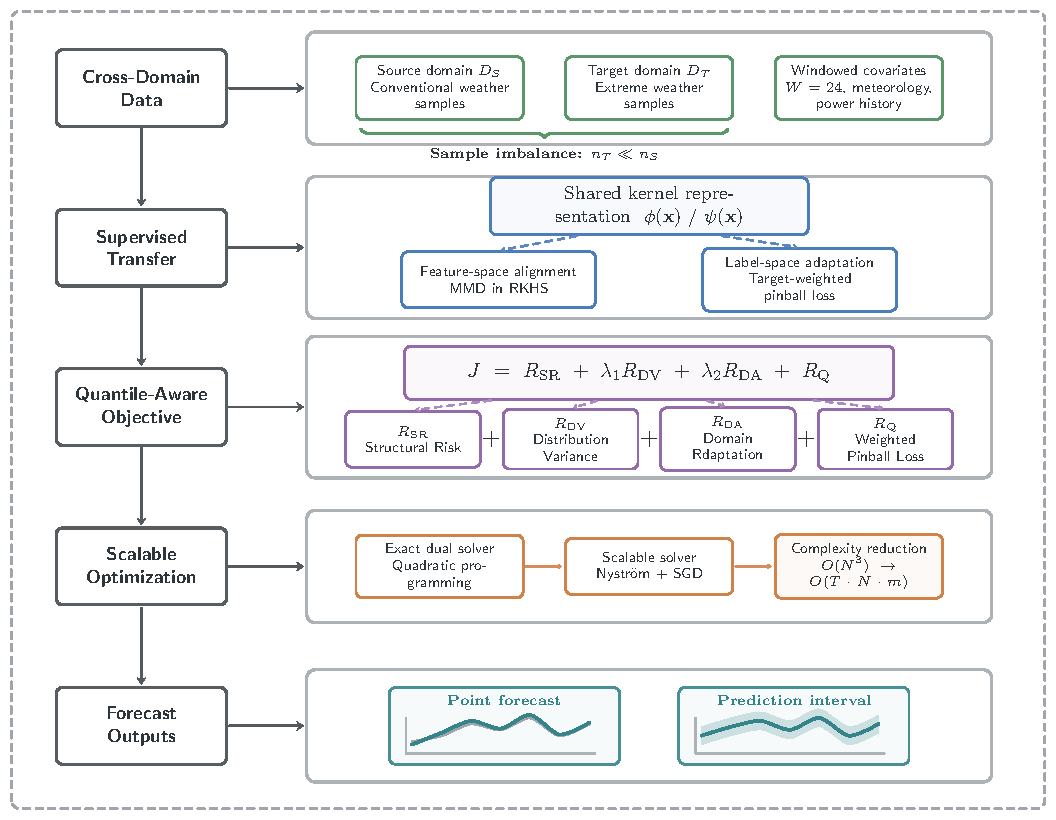
\includegraphics[width=\textwidth]{build/framework.pdf}
\caption{Overall architecture of the proposed TL-QLDMR model.}
\label{fig:framework}
\end{figure}

% The left column shows the five-stage pipeline: cross-domain data preparation, supervised transfer learning, quantile-aware objective construction, scalable optimization, and forecast outputs. Each stage is elaborated in the corresponding right panel. In the supervised transfer stage, the shared kernel representation branches into feature-space alignment via MMD in RKHS and label-space adaptation via target-weighted pinball loss (indicated by dashed arrows). The quantile-aware objective decomposes into four additive terms: structural risk $R_{\mathrm{SR}}$, distribution variance $R_{\mathrm{DV}}$, domain adaptation $R_{\mathrm{DA}}$, and weighted pinball loss $R_{\mathrm{Q}}$. The optimization stage provides both an exact dual QP solver and a scalable Nystr\"om-SGD solver with complexity reduction from $O(N^3)$ to $O(T \cdot N \cdot m)$. The final outputs include deterministic point forecasts and probabilistic prediction intervals.

\subsubsection{Objective Function}
Our optimization goal is to find the optimal $\boldsymbol{w}, b$ and slack variables $\boldsymbol{\xi}, \boldsymbol{\xi}^*$ to minimize the following objective function $J$. Let $\bar{u}_S = \frac{1}{n_S}\sum_{i=1}^{n_S}(y_{S,i} - f(\boldsymbol{x}_{S,i}))$ denote the mean residual over the source domain, which is treated as a scalar constant during optimization
\begin{equation}
\label{eq:objective}
\begin{aligned}
\min_{\boldsymbol{w}, b, \boldsymbol{\xi}, \boldsymbol{\xi}^*} \quad J = & \underbrace{\frac{1}{2} \|\boldsymbol{w}\|^2}_{\text{(1) Structural Risk}} \\
& + \underbrace{\lambda_1 \sum_{i=1}^{n_S} \left( (y_{S,i} - \boldsymbol{w}^T\phi(\boldsymbol{x}_{S,i}) - b) - \bar{u}_S \right)^2}_{\text{(2) Distribution Variance}} \\
& + \underbrace{\lambda_2 \left\| \frac{1}{n_S} \sum_{i=1}^{n_S} \phi(\boldsymbol{x}_{S,i}) - \frac{1}{n_T} \sum_{j=1}^{n_T} \phi(\boldsymbol{x}_{T,j}) \right\|_{\mathcal{H}}^2}_{\text{(3) Domain Adaptation}} \\
& + \underbrace{C_S \sum_{i=1}^{n_S} L_{\tau}(y_{S,i}, f(\boldsymbol{x}_{S,i})) + C_T \sum_{j=1}^{n_T} L_{\tau}(y_{T,j}, f(\boldsymbol{x}_{T,j}))}_{\text{(4) Weighted Pinball Loss}},
\end{aligned}
\end{equation}
the physical meaning of each term is as follows:
\begin{enumerate}
    \item \textbf{Structural Risk}: This term controls the complexity of the model and prevents overfitting, embodying the maximum margin principle of SVM.
    \item \textbf{Distribution Variance}: This term is the core of our proposed Quantile LDMR model, incorporating a critical modification to the original LDMR variance.
    \begin{itemize}
        \item \textbf{Theoretical Conflict}: The original LDMR minimizes the variance of residuals, which implicitly encourages a symmetric, concentrated error distribution around zero. However, quantile regression at level $\tau \neq 0.5$ requires an asymmetric residual distribution where approximately $\tau$ proportion of errors are negative. Applying a symmetric variance penalty would force the residual distribution towards symmetry, degrading the skewness required for accurate quantile estimation.
        \item \textbf{Asymmetric Modification}: To resolve this, we employ an asymmetric variance regularization based on the algebraic residuals. This design allows the model to reduce error dispersion without constraining the distribution's direction, thereby preserving the non-symmetric properties essential for the Pinball Loss and improving interval coverage.
    \end{itemize}
    \item \textbf{Domain Adaptation (MMD)}: This term aligns source and target domains by penalizing the projected mean discrepancy in RKHS. This alignment ensures that the learned predictor is robust to the feature-space shift between normal and extreme-event regimes. MMD is chosen because it is non-parametric, computationally tractable, and directly compatible with kernelized optimization.
    \item \textbf{Weighted Pinball Loss}: This term performs label-space adaptation under sample imbalance. Unlike purely unsupervised alignment, the objective explicitly includes target-domain labels:
    \begin{itemize}
        \item \textbf{Label-supervised correction}: extreme-event target labels constrain the model in regions where source-domain trends are no longer reliable (e.g., high wind speed under cut-out operation).
        \item \textbf{Imbalance-aware weighting}: by setting $C_T \gg C_S$, prediction errors on scarce target samples receive stronger penalties, preventing optimization from being dominated by abundant source samples.
    \end{itemize}
\end{enumerate}

\subsubsection{Constraints}
To handle the non-differentiability of the pinball loss, we introduce slack variables $\xi_k, \xi_k^*$ to transform it into linear constraints. These constraints apply uniformly to all samples $k$ in the combined training set $D = D_S \cup D_T$, while domain-specific weighting is handled through $C_S$ and $C_T$ in the objective function
\begin{equation}
\label{eq:constraints}
\begin{cases}
y_k - (\boldsymbol{w}^T\phi(\boldsymbol{x}_k) + b) \le \xi_k, & \forall k \in \{1, \dots, n_S + n_T\} \\
(\boldsymbol{w}^T\phi(\boldsymbol{x}_k) + b) - y_k \le \xi_k^*, & \forall k \in \{1, \dots, n_S + n_T\} \\
\xi_k \ge 0, \quad \xi_k^* \ge 0
\end{cases},
\end{equation}
in the objective function, the term $L_{\tau}(y_k, f(\boldsymbol{x}_k))$ corresponds to $\tau \xi_k + (1-\tau) \xi_k^*$.

\subsection{Model Optimization}\label{optimization}
This section derives the dual problem of TL-QLDMR to enable efficient solution via QP.

\subsubsection{Matrix Reformulation of the Primal Problem}
To facilitate the derivation, the variance term and the MMD term in the objective function [Eq. (\ref{eq:objective})] are rewritten using matrix traces or norms. Let $X = [\boldsymbol{X}_S, \boldsymbol{X}_T]$ denote the entire training set with $N = n_S + n_T$ samples.
For consistency with standard derivations, a coefficient of $1/2$ is added to the variance and MMD terms. The primal objective can be reformulated as
\begin{equation}
\label{eq:primal_matrix}
\min_{\boldsymbol{w}, b, \boldsymbol{\xi}, \boldsymbol{\xi}^*} \quad \frac{1}{2} \|\boldsymbol{w}\|^2 + \frac{\lambda_1}{2} \text{Var}_S(\boldsymbol{w}, b) + \frac{\lambda_2}{2} \text{MMD}^2(\boldsymbol{w}) + \sum_{k=1}^N C_k L_\tau(y_k, f(\boldsymbol{x}_k)),
\end{equation}
where $C_k$ takes value $C_S$ if sample $k \in D_S$ and $C_T$ if $k \in D_T$.

Two auxiliary matrices are introduced to express the variance and MMD terms in Eq. (\ref{eq:primal_matrix}) as quadratic forms of the weights:
\begin{enumerate}
    \item \textbf{Variance Matrix} $\mathbf{S}$: To represent the source-domain variance $\sum_{i \in D_S} (y_{S,i} - f(\boldsymbol{x}_{S,i}) - \bar{u}_S)^2$, we define a centering matrix $\boldsymbol{H}_S = \boldsymbol{I}_{n_S} - \frac{1}{n_S} \boldsymbol{1}_{n_S} \boldsymbol{1}_{n_S}^T$. The variance term can be written as $\| \boldsymbol{H}_S (\boldsymbol{y}_S - \boldsymbol{f}_S) \|^2$. To extend this to the full dataset, we define an $N \times N$ matrix $\mathbf{S}$
    \begin{equation}
    \label{eq:matrix_S}
    \mathbf{S} = \begin{bmatrix} \boldsymbol{H}_S & \mathbf{0} \\ \mathbf{0} & \mathbf{0} \end{bmatrix}.
    \end{equation}
    \item \textbf{MMD Matrix} $\mathbf{M}$: The domain-adaptation term represents the squared difference between projected source and target means. We define the MMD coefficient matrix $\mathbf{M} \in \mathbb{R}^{N \times N}$ as
    \begin{equation}
    \label{eq:matrix_M}
    M_{ij} = \begin{cases} \frac{1}{n_S^2} & i,j \in D_S \\ \frac{1}{n_T^2} & i,j \in D_T \\ \frac{-1}{n_S n_T} & \text{otherwise} \end{cases}.
    \end{equation}
\end{enumerate}

\subsubsection{Representer Theorem and Kernelization}
According to the representer theorem (\cite{scholkopf2001representer}), the optimal weight vector $\boldsymbol{w}$ lies in the span of the feature mappings of the training samples. Note that the representer theorem applies here because all regularization terms (structural risk, variance, and MMD) can be expressed as functions of inner products in RKHS, preserving the kernel structure. Therefore
\begin{equation}
\label{eq:representer}
\boldsymbol{w} = \sum_{i=1}^{N} \beta_i \phi(\boldsymbol{x}_i) = \boldsymbol{\Phi} \boldsymbol{\beta},
\end{equation}
where $\boldsymbol{\Phi} = [\phi(\boldsymbol{x}_1), \dots, \phi(\boldsymbol{x}_N)]$ is the feature matrix and $\boldsymbol{\beta} = [\beta_1, \dots, \beta_N]^T$ are the coefficients.
Substituting Eq. (\ref{eq:representer}) into the prediction function, we get $f(\boldsymbol{X}) = \boldsymbol{\beta}^T \boldsymbol{K} + b \boldsymbol{1}^T$, where $\boldsymbol{K} = \boldsymbol{\Phi}^T \boldsymbol{\Phi}$ is the $N \times N$ kernel matrix.
Consequently, using Eq. (\ref{eq:matrix_S}) and Eq. (\ref{eq:matrix_M}), the structural risk, variance, and MMD terms can be expressed in terms of $\boldsymbol{\beta}$:
\begin{itemize}
    \item Structural Risk: $\|\boldsymbol{w}\|^2 = \boldsymbol{\beta}^T \boldsymbol{K} \boldsymbol{\beta}$.
    \item Distribution Variance: The quadratic part with respect to $\boldsymbol{\beta}$ is $\boldsymbol{\beta}^T \boldsymbol{K} \mathbf{S} \boldsymbol{K} \boldsymbol{\beta}$. Note that the bias $b$ is eliminated by the centering matrix $\boldsymbol{H}_S$.
    \item Domain Adaptation (MMD): $\text{MMD}^2(\boldsymbol{w}) = \boldsymbol{\beta}^T \boldsymbol{K} \mathbf{M} \boldsymbol{K} \boldsymbol{\beta}$.
\end{itemize}

Combining these, we define the total coefficient matrix $\boldsymbol{\Omega}$
\begin{equation}
\label{eq:Omega}
\boldsymbol{\Omega} = \boldsymbol{K} + \lambda_1 \boldsymbol{K} \mathbf{S} \boldsymbol{K} + \lambda_2 \boldsymbol{K} \mathbf{M} \boldsymbol{K}.
\end{equation}

\begin{remark}
When $\boldsymbol{K}$ is positive definite (which holds for common kernels such as RBF on distinct samples) and $\lambda_1, \lambda_2 > 0$, the matrix $\boldsymbol{\Omega}$ is positive definite. This ensures that $\boldsymbol{\Omega}$ is invertible and the optimization problem is well-posed. The positive definiteness of $\boldsymbol{\Omega}$ also guarantees the strong convexity of the objective function, which is essential for both the dual QP formulation and the convergence analysis of the scalable SGD algorithm.
\end{remark}
By substituting the kernelized terms and Eq. (\ref{eq:Omega}) into Eq. (\ref{eq:primal_matrix}), the kernelized primal problem becomes (ignoring constant terms w.r.t $b$ in variance)
\begin{equation}
\label{eq:kernel_primal}
\min_{\boldsymbol{\beta}, b, \boldsymbol{\xi}, \boldsymbol{\xi}^*} \quad \frac{1}{2} \boldsymbol{\beta}^T \boldsymbol{\Omega} \boldsymbol{\beta} - (\lambda_1 \boldsymbol{K} \mathbf{S} \boldsymbol{Y})^T \boldsymbol{\beta} + \sum_{k=1}^N C_k (\tau \xi_k + (1-\tau)\xi_k^*),
\end{equation}
subject to the constraints from Eq. (\ref{eq:constraints})
\begin{equation}
\label{eq:kernel_constraints}
y_k - (\boldsymbol{K}_k \boldsymbol{\beta} + b) \le \xi_k, \quad (\boldsymbol{K}_k \boldsymbol{\beta} + b) - y_k \le \xi_k^*, \quad \xi_k, \xi_k^* \ge 0.
\end{equation}

\subsubsection{Lagrangian and Dual Problem}
We introduce Lagrange multipliers $\alpha_k, \alpha_k^*, \mu_k, \mu_k^* \ge 0$ for Eq. (\ref{eq:kernel_constraints}). The Lagrangian function $\mathcal{L}$ is constructed as
\begin{equation}
\label{eq:lagrangian}
\begin{aligned}
\mathcal{L} = &\frac{1}{2} \boldsymbol{\beta}^T \boldsymbol{\Omega} \boldsymbol{\beta} - (\lambda_1 \boldsymbol{K} \mathbf{S} \boldsymbol{Y})^T \boldsymbol{\beta} + \sum_{k=1}^N C_k (\tau \xi_k + (1-\tau)\xi_k^*) \\
&- \sum_{k=1}^N \alpha_k (\xi_k - y_k + \boldsymbol{K}_k \boldsymbol{\beta} + b) - \sum_{k=1}^N \alpha_k^* (\xi_k^* + y_k - \boldsymbol{K}_k \boldsymbol{\beta} - b) - \sum (\mu_k \xi_k + \mu_k^* \xi_k^*),
\end{aligned}
\end{equation}
by setting the partial derivatives of Eq. (\ref{eq:lagrangian}) with respect to the primal variables ($b, \boldsymbol{\xi}, \boldsymbol{\xi}^*, \boldsymbol{\beta}$) to zero, along with the complementary slackness and primal feasibility conditions, we obtain the KKT conditions
\begin{align}
    \label{eq:kkt_b} \frac{\partial \mathcal{L}}{\partial b} = 0 & \implies \sum_{k=1}^N (\alpha_k - \alpha_k^*) = 0 \\
    \label{eq:kkt_xi} \frac{\partial \mathcal{L}}{\partial \xi_k} = 0, \frac{\partial \mathcal{L}}{\partial \xi_k^*} = 0 & \implies \alpha_k \in [0, C_k \tau], \quad \alpha_k^* \in [0, C_k (1-\tau)] \\
    \label{eq:kkt_beta} \frac{\partial \mathcal{L}}{\partial \boldsymbol{\beta}} = 0 & \implies \boldsymbol{\Omega} \boldsymbol{\beta} - \lambda_1 \boldsymbol{K} \mathbf{S} \boldsymbol{Y} - \boldsymbol{K} (\boldsymbol{\alpha} - \boldsymbol{\alpha}^*) = 0,
\end{align}
let $\boldsymbol{\gamma} = \boldsymbol{\alpha} - \boldsymbol{\alpha}^*$. From Eq. (\ref{eq:kkt_beta}), the optimal $\boldsymbol{\beta}$ is derived as
\begin{equation}
\label{eq:beta_optimal}
\boldsymbol{\beta} = \boldsymbol{\Omega}^{-1} (\boldsymbol{K} \boldsymbol{\gamma} + \lambda_1 \boldsymbol{K} \mathbf{S} \boldsymbol{Y}).
\end{equation}

Substituting Eq. (\ref{eq:beta_optimal}) back into Eq. (\ref{eq:lagrangian}), and simplifying using Eq. (\ref{eq:kkt_b}) and Eq. (\ref{eq:kkt_xi}), we arrive at the dual problem, which is a standard QP problem
\begin{equation}
\label{eq:dual_problem}
\begin{aligned}
\min_{\boldsymbol{\alpha}, \boldsymbol{\alpha}^*} \quad & \frac{1}{2} (\boldsymbol{\alpha} - \boldsymbol{\alpha}^*)^T \mathbf{Q}_{dual} (\boldsymbol{\alpha} - \boldsymbol{\alpha}^*) + \mathbf{p}_{dual}^T (\boldsymbol{\alpha} - \boldsymbol{\alpha}^*) \\
\text{s.t.} \quad & \sum_{k=1}^N (\alpha_k - \alpha_k^*) = 0 \\
& 0 \le \alpha_k \le C_k \tau, \quad \forall k \\
& 0 \le \alpha_k^* \le C_k (1-\tau), \quad \forall k
\end{aligned},
\end{equation}
where the dual matrix $\mathbf{Q}_{dual}$ and vector $\mathbf{p}_{dual}$ are defined as
\begin{equation}
\label{eq:dual_matrices}
\mathbf{Q}_{dual} = \boldsymbol{K} \boldsymbol{\Omega}^{-1} \boldsymbol{K}, \quad \mathbf{p}_{dual} = \lambda_1 \boldsymbol{K} \boldsymbol{\Omega}^{-1} \boldsymbol{K} \mathbf{S} \boldsymbol{Y} - \boldsymbol{Y}.
\end{equation}

Once the optimal $\boldsymbol{\alpha}, \boldsymbol{\alpha}^*$ are found using a QP solver for Eq. (\ref{eq:dual_problem}), we can recover $\boldsymbol{\beta}$ using Eq. (\ref{eq:beta_optimal}) and construct the final decision function $f(\boldsymbol{x})$.


\subsection{Scalable Optimization via Nystr\"{o}m Approximation}\label{fast_alg}
The standard QP-based solver incurs $O(N^3)$ complexity due to full kernel-matrix computation and inversion, which becomes prohibitive for large-scale datasets. To address this, we develop a scalable Nystr\"{o}m-SGD algorithm that reduces the complexity to $O(T \cdot N \cdot m)$, where $T$ is the number of SGD iterations and $m \ll N$ is the number of landmark points.

To keep the scalable solver consistent with the exact kernelized problem in Eq. (\ref{eq:kernel_primal}), we replace the implicit RKHS mapping $\phi(\boldsymbol{x})$ with an explicit $m$-dimensional Nystr\"{o}m feature map. We select $m$ landmark points $Z = \{z_1, \ldots, z_m\}$ from the combined training set $D = D_S \cup D_T$ via K-Means clustering \citep{zhang2010clustered}. Let $\boldsymbol{W} \in \mathbb{R}^{m \times m}$ denote the kernel matrix among landmarks, where $W_{ij} = k(z_i, z_j)$. The explicit feature mapping $\psi: \mathcal{X} \to \mathbb{R}^m$ is
\begin{equation}
\label{eq:nystrom_feature}
\psi(\boldsymbol{x}) = \boldsymbol{W}^{-1/2} [k(\boldsymbol{x}, z_1), \ldots, k(\boldsymbol{x}, z_m)]^T,
\end{equation}
where $\boldsymbol{W}^{-1/2}$ is computed via eigendecomposition, satisfying $k(\boldsymbol{x}_i, \boldsymbol{x}_j) \approx \psi(\boldsymbol{x}_i)^T \psi(\boldsymbol{x}_j)$.

With the explicit features, the prediction becomes $f(\boldsymbol{x}) = \boldsymbol{w}^T \psi(\boldsymbol{x}) + b$, where $\boldsymbol{w} \in \mathbb{R}^m$. Let $\boldsymbol{\Psi}_S \in \mathbb{R}^{n_S \times m}$ and $\boldsymbol{\Psi}_T \in \mathbb{R}^{n_T \times m}$ denote the mapped feature matrices, and define $\Delta_{\psi} = \bar{\boldsymbol{\psi}}_S - \bar{\boldsymbol{\psi}}_T$. The Nystr\"{o}m approximation of Eq. (\ref{eq:kernel_primal}) is
\begin{equation}
\label{eq:nystrom_primal}
\min_{\boldsymbol{w}, b} \quad \frac{1}{2}\boldsymbol{w}^T \boldsymbol{R} \boldsymbol{w} - \boldsymbol{c}^T \boldsymbol{w}
+ C_S \sum_{i=1}^{n_S} L_{\tau}(y_{S,i}, f(\boldsymbol{x}_{S,i}))
+ C_T \sum_{j=1}^{n_T} L_{\tau}(y_{T,j}, f(\boldsymbol{x}_{T,j})),
\end{equation}
where the regularization matrix $\boldsymbol{R} \in \mathbb{R}^{m \times m}$ is
\begin{equation}
\label{eq:reg_matrix}
\boldsymbol{R} = \boldsymbol{I} + \lambda_1 \boldsymbol{\Psi}_S^T \boldsymbol{H}_S \boldsymbol{\Psi}_S + \lambda_2 \Delta_{\psi}\Delta_{\psi}^T,
\end{equation}
and the linear term induced by the source-domain variance is
\begin{equation}
\label{eq:nystrom_linear}
\boldsymbol{c} = \lambda_1 \boldsymbol{\Psi}_S^T \boldsymbol{H}_S \boldsymbol{y}_S.
\end{equation}

Here $\boldsymbol{H}_S = \boldsymbol{I}_{n_S} - \frac{1}{n_S} \boldsymbol{1}_{n_S} \boldsymbol{1}_{n_S}^T$ is the centering matrix. Therefore, the scalable solver preserves the same four components as the exact formulation: structural risk, source-domain variance regularization, MMD-based alignment, and weighted pinball loss. The only change is that optimization is performed in an explicit $m$-dimensional feature space instead of the $N$-dimensional dual coefficient space.

For each sample $k$ in a mini-batch $\mathcal{B}$, a valid subgradient of the pinball loss with respect to the prediction $\hat{y}_k = f(\boldsymbol{x}_k)$ is
\begin{equation}
\label{eq:subgradient}
g_k \in \partial_{\hat{y}_k} L_{\tau}(y_k, \hat{y}_k)= \begin{cases}
    1-\tau, & \text{if } \hat{y}_k > y_k, \\
    [-\tau,\, 1-\tau], & \text{if } \hat{y}_k = y_k, \\
    -\tau, & \text{if } \hat{y}_k < y_k.
\end{cases}
\end{equation}

In implementation, we use $g_k = 1-\tau$ when $\hat{y}_k > y_k$ and $g_k = -\tau$ otherwise. The weighted subgradient $\tilde{g}_k = C_k g_k$ (where $C_k \in \{C_S, C_T\}$) yields the stochastic gradients
\begin{equation}
\label{eq:param_gradients}
\nabla_{\boldsymbol{w}} J = \boldsymbol{R} \boldsymbol{w} - \boldsymbol{c} + \frac{1}{|\mathcal{B}|} \sum_{k \in \mathcal{B}} \tilde{g}_k \psi(\boldsymbol{x}_k), \quad \nabla_b J = \frac{1}{|\mathcal{B}|} \sum_{k \in \mathcal{B}} \tilde{g}_k.
\end{equation}

The complete procedure is summarized in Algorithm \ref{alg:fast_TL-QLDMR}. The overall time complexity is $O(T \cdot N \cdot m + m^3)$. Since $m \ll N$, this represents a substantial reduction from the $O(N^3)$ complexity of the standard QP solver. Table \ref{tab:complexity} summarizes the comparison.

\begin{algorithm}[t]
\SetKwInOut{Input}{Input}
\SetKwInOut{Output}{Output}
\caption{TL-QLDMR via Nystr\"{o}m-SGD}
\label{alg:fast_TL-QLDMR}
\Input{Source data $D_S$, Target data $D_T$, Number of landmarks $m$, Quantile $\tau$, Hyperparameters $\lambda_1, \lambda_2, C_S, C_T$, Learning rate $\eta$, Batch size $B$, Max iterations $T$.}
\Output{Optimal weights $\boldsymbol{w} \in \mathbb{R}^m$ and bias $b \in \mathbb{R}$.}

\tcp{Step 1: Nystr\"{o}m Feature Mapping}
Select $m$ landmarks $Z = \{z_1, \ldots, z_m\}$ from $D = D_S \cup D_T$ via K-Means\;
Compute landmark kernel matrix $\boldsymbol{W} \in \mathbb{R}^{m \times m}$\;
Compute $\boldsymbol{W}^{-1/2}$ via eigendecomposition\;
Construct explicit features $\psi(\boldsymbol{x})$ for all samples using Eq. \eqref{eq:nystrom_feature}\;

\tcp{Step 2: Pre-compute Regularization Matrix}
Compute feature matrices $\boldsymbol{\Psi}_S$, $\boldsymbol{\Psi}_T$, domain means $\bar{\boldsymbol{\psi}}_S$, $\bar{\boldsymbol{\psi}}_T$, and vector $\boldsymbol{c}$ in Eq. \eqref{eq:nystrom_linear}\;
Construct regularization matrix $\boldsymbol{R}$ using Eq. \eqref{eq:reg_matrix}\;

\tcp{Step 3: Stochastic Optimization}
Initialize $\boldsymbol{w} \leftarrow \boldsymbol{0}$, $b \leftarrow 0$\;
\For{$t = 1$ \KwTo $T$}{
    Shuffle combined dataset $D = D_S \cup D_T$\;
    \For{each mini-batch $\mathcal{B} \subset D$}{
        Compute predictions: $\hat{y}_k = \boldsymbol{w}^T \psi(\boldsymbol{x}_k) + b$, $\forall k \in \mathcal{B}$\;
        Compute sub-gradients $g_k$ using Eq. \eqref{eq:subgradient}\;
        Apply sample weights: $\tilde{g}_k \leftarrow C_k \cdot g_k$\;
        Compute gradients $\nabla_{\boldsymbol{w}} J$, $\nabla_b J$ using Eq. \eqref{eq:param_gradients}\;
        Update $\boldsymbol{w} \leftarrow \boldsymbol{w} - \eta \nabla_{\boldsymbol{w}} J$ and $b \leftarrow b - \eta \nabla_b J$\;
    }
}
\Return $\boldsymbol{w}$, $b$\;
\end{algorithm}


\begin{table}[htbp]
\centering
\caption{Complexity comparison between standard QP and scalable algorithm}
\label{tab:complexity}
\begin{tabular}{lcc}
\toprule
\textbf{Component} & \textbf{Standard QP} & \textbf{Scalable (Ours)} \\
\midrule
Kernel/Feature Computation & $O(N^2 d)$ & $O(N m d)$ \\
Matrix Inversion & $O(N^3)$ & $O(m^3)$ \\
Optimization & $O(N^3)$ & $O(T N m)$ \\
\midrule
\textbf{Total} & $O(N^3)$ & $O(T N m + m^3)$ \\
\bottomrule
\end{tabular}
\end{table}

The correspondence with the exact QP route is therefore explicit: Eq. (\ref{eq:nystrom_primal}) is the Nystr\"{o}m-feature counterpart of Eq. (\ref{eq:kernel_primal}), and Eqs. (\ref{eq:reg_matrix})--(\ref{eq:param_gradients}) preserve the same structural terms after replacing the implicit kernel representation with a low-rank explicit one. Moreover, $\boldsymbol{R}$ is positive definite because $\boldsymbol{I}$ is positive definite and the remaining two matrices are positive semi-definite. Hence the approximate primal objective is strongly convex, and SGD converges to the global optimum at a rate of $O(1/T)$ under a decaying step-size schedule \citep{bottou2018optimization}. As the number of landmarks increases, the Nystr\"{o}m approximation becomes increasingly faithful to the exact kernel matrix, so the scalable solution approaches that of the exact QP solver \citep{kumar2012sampling, zhang2010clustered}.


%------------------------- Experiments --------------------%
\section{Experiments}\label{Experiments}

In this section, we conduct a comprehensive experimental evaluation of the proposed TL-QLDMR model for wind power forecasting in the extreme-event domain. The experiments are organized into five progressive stages: (1) extreme-event sample screening and domain shift quantification across multiple wind farms (Section~\ref{sec:exp1}); (2) deterministic point prediction comparison on the wind farm exhibiting the most severe distribution shift (Section~\ref{sec:exp2}); (3) probabilistic interval prediction evaluation under a 95\% confidence level (Section~\ref{sec:exp3}); (4) ablation study to validate the contribution of each core component (Section~\ref{sec:exp4}); and (5) scalable optimization validation to assess the computational efficiency of the proposed Nystr\"{o}m-SGD solver (Section~\ref{sec:exp5}).

%---------------- Dataset Description --------------------%
\subsection{Dataset Description}\label{sec:data}

The experiments are conducted on a publicly available wind farm SCADA dataset published by the State Grid Renewable Energy Generation Dataset \citep{s41597-022-01696-6}. The dataset contains records from six onshore wind farms with nominal capacities ranging from 36\,MW to 200\,MW. Each record is sampled at 15-minute intervals and includes the following meteorological and operational variables:

\begin{itemize}
    \item Wind speed at multiple heights: hub height, 50\,m, 30\,m, and 10\,m (m/s);
    \item Wind direction at hub height (degrees);
    \item Air temperature ($^\circ$C);
    \item Atmospheric pressure (hPa);
    \item Relative humidity (\%);
    \item Active power output (MW).
\end{itemize}

Table~\ref{tab:farm_summary} summarizes the basic characteristics of the six wind farms. Each farm contains approximately 70{,}000 time-stamped records spanning multiple years of continuous operation.

\begin{table}[ht]
\centering
\caption{Summary of wind farm sites used in the experiments.}
\setlength{\tabcolsep}{4mm}
\begin{tabular}{cccc}
\toprule
Farm ID & Site Name & Nominal Capacity (MW) & Total Samples \\
\midrule
1 & Wind farm site 1 & 99  & $\sim$70{,}000 \\
2 & Wind farm site 2 & 200 & $\sim$70{,}000 \\
3 & Wind farm site 3 & 99  & $\sim$70{,}000 \\
4 & Wind farm site 4 & 66  & $\sim$70{,}000 \\
5 & Wind farm site 5 & 36  & $\sim$70{,}000 \\
6 & Wind farm site 6 & 96  & $\sim$70{,}000 \\
\bottomrule
\end{tabular}
\label{tab:farm_summary}
\end{table}

%---------------- Extreme-Event Domain Definition --------------------%
\subsection{Extreme-Event Domain Definition}\label{sec:extreme_def}

A critical prerequisite for evaluating transfer learning under extreme conditions is the rigorous definition of what constitutes an ``extreme event'' in wind power forecasting \citep{sideratos2012extreme, liu2024extreme}. In this study, extreme events do not denote a single named meteorological subtype, such as typhoon, icing, or a specific ramping pattern. Instead, they refer to a unified target domain composed of rare, high-risk, high-volatility, and out-of-distribution operating states induced by extreme meteorological deviations and their associated turbine responses relative to the normal-operating domain, consistent with transfer-learning settings in which the source and target domains differ through their marginal distributions and operational regimes \citep{pan2010survey, bendavid2010theory}. To construct this target domain, a physics-statistics hybrid screening strategy is adopted: physical thresholding captures deterministic high-wind shutdown risk, whereas percentile-based rules identify statistically rare meteorological deviations at each wind farm, following the broader logic of mixed rule-and-statistics criteria used in recent extreme-event energy data studies \citep{liu2023eweld}. A sample is classified as belonging to the target domain if it satisfies any of the following criteria:

\begin{enumerate}
    \item \textbf{Statistical wind speed extreme}: Hub-height wind speed exceeds the 98th percentile of the farm's historical distribution;
    \item \textbf{Temperature extreme}: Air temperature falls below the 2nd percentile or exceeds the 98th percentile;
    \item \textbf{Cut-out wind speed}: Hub-height wind speed exceeds 25\,m/s, the typical cut-out threshold for modern wind turbines.
\end{enumerate}

The 25\,m/s threshold is treated here as a nominal cut-out speed. Although the exact cut-out point may vary slightly across turbine types, values around 25\,m/s are widely used in wind turbine power-curve characterization as the shutdown region associated with safety protection \citep{rabanal2019midas}. This threshold is therefore sufficient to capture the core methodological feature of high-wind-induced nonlinear shutdown risk. Notably, the power ramp criterion (rapid power fluctuations exceeding 5\% of nominal capacity per 15-minute interval) is deliberately excluded from the extreme definition. This design choice avoids conflating control-induced power curtailment or dispatch adjustments with genuinely weather-driven anomalies.

No further subdivision of extreme-event samples into multiple subclasses is attempted. This choice is deliberate because extreme events are inherently scarce in realistic forecasting settings; splitting them into fine-grained categories would substantially weaken the statistical support available for transfer learning and would turn a small-sample problem into a near-few-shot problem, a difficulty also reported in recent extreme-condition wind power studies \citep{liang2025coldwave}. From the perspective of domain adaptation, these heterogeneous extreme states share the same modeling characteristic: they are all out-of-distribution samples exhibiting elevated volatility, non-stationarity, and clear deviation from normal operating patterns \citep{pan2010survey, bendavid2010theory}. The objective of TL-QLDMR is therefore to learn a unified disturbance-robust adaptation mechanism rather than a separate submodel for each rare event type. The union of the above three rules thus forms a single target domain that is physically interpretable, statistically sufficient for model training, and consistent with the data-scarce nature of extreme-event forecasting. All remaining samples constitute the normal-operating source domain.

%---------------- Experimental Setup --------------------%
\subsection{Experimental Setup}\label{sec:setup}

For deterministic point prediction, we employ Root Mean Squared Error (RMSE), Mean Absolute Error (MAE), and the Coefficient of Determination ($R^2$) as evaluation metrics. RMSE and MAE quantify the magnitude of prediction errors, while $R^2$ measures the proportion of variance explained by the model. For probabilistic interval prediction, we adopt Prediction Interval Coverage Probability (PICP), Mean Prediction Interval Width (MPIW), Prediction Interval Normalized Average Width (PINAW), Coverage Width-based Criterion (CWC), and Winkler Score.

To quantify the distribution discrepancy between the normal-operating and extreme-event domains, we employ two complementary metrics computed on both wind speed and power dimensions: the Wasserstein-1 distance ($W_1$), which measures the minimum transportation cost to transform one distribution into the other, and the Kolmogorov--Smirnov statistic (KS), which captures the supremum of the absolute difference between the empirical cumulative distribution functions of the two domains.

The hyperparameters of TL-QLDMR are selected by validation-based tuning within each experiment. The searched ranges are logarithmic grids for $\lambda_1$ and $\lambda_2$ from $10^{-6}$ to $10^{6}$, $C_S \in \{0.05, 0.1, 0.2\}$, $C_T \in \{50, 300, 1000\}$, and kernel bandwidth $\gamma \in \{2^{-6}, \ldots, 2^{6}\}$. The Nystr\"{o}m-SGD solver is tuned over landmark size $m \in [800, 1500]$, learning rate in $\{0.005, 0.01\}$, and training epochs in $[48, 80]$, with mini-batch size fixed at 256. All experiments are implemented in Python and executed on a GPU server equipped with eight NVIDIA Tesla V100-SXM2-32GB GPUs (32\,GB memory per GPU), using NVIDIA driver version 550.54.15 and CUDA 12.4. All random splits use a fixed seed for reproducibility.


%---------------- Experiment 1 --------------------%
\subsection{Experiment 1: Extreme-Event Sample Screening and Domain Shift Quantification}\label{sec:exp1}

The first experiment identifies extreme-event samples across all six wind farms using the criteria in Section~\ref{sec:extreme_def}, and then quantifies source-target distribution shift for each farm. Table~\ref{tab:exp1_shift} reports the domain-shift statistics sorted by the composite Wasserstein distance $W_1(\text{wind}) + W_1(\text{power})$. Preliminary sensitivity checks show that a stricter 99th-percentile wind-speed rule leaves too few target-domain samples for stable model development, whereas the adopted 98th-percentile rule preserves event extremity while maintaining statistical sufficiency.

\begin{table*}[ht]
\centering
\caption{Domain shift metrics between normal-operating and extreme-event domains across six wind farms. Farms are sorted by the composite Wasserstein distance in descending order.}
\setlength{\tabcolsep}{3mm}
\begin{tabular}{lccccc}
\toprule
Wind Farm & Extreme-Event Samples & $W_1$(Wind) & $W_1$(Power) & KS(Wind) & KS(Power) \\
\midrule
Farm 6 (96\,MW)  & 4{,}144 & 4.060 & 21.057 & 0.389 & 0.344 \\
Farm 3 (99\,MW)  & 4{,}144 & 3.389 & 18.915 & 0.338 & 0.265 \\
Farm 2 (200\,MW) & 4{,}211 & 3.467 & 16.166 & 0.333 & 0.142 \\
Farm 5 (36\,MW)  & 3{,}039 & 4.195 &  9.851 & 0.460 & 0.363 \\
Farm 4 (66\,MW)  & 4{,}046 & 4.235 &  7.759 & 0.347 & 0.201 \\
Farm 1 (99\,MW)  & 4{,}184 & 3.140 &  5.964 & 0.335 & 0.116 \\
\bottomrule
\end{tabular}
\label{tab:exp1_shift}
\end{table*}

Fig.~\ref{fig:domain_shift} visualizes the distribution shift between normal-operating and extreme-event domains for all six wind farms. Each subplot displays the kernel density estimates of wind speed (upper panel) and power output (lower panel) for both domains. The visual comparison confirms the quantitative findings in Table~\ref{tab:exp1_shift}: Farm~6 exhibits the most pronounced separation between the two distributions, particularly in the power dimension, where the extreme-event domain shows a bimodal pattern with substantial mass near zero power (cut-out events) and high power (pre-cut-out high wind conditions).

Several observations emerge from Table~\ref{tab:exp1_shift} and Fig.~\ref{fig:domain_shift}. First, all six farms exhibit non-trivial distribution shifts between the normal-operating and extreme-event domains, with KS statistics ranging from 0.116 to 0.460, confirming that extreme events induce statistically significant distributional changes in both wind speed and power output. Second, the magnitude of the power distribution shift varies substantially across farms: Farm~6 exhibits a Wasserstein distance of 21.057 in the power dimension, approximately 3.5 times that of Farm~1 (5.964). This disparity reflects differences in turbine control strategies, terrain effects, and the local meteorological characteristics of each site.

Farm~6 (nominal capacity 96\,MW) ranks first in the composite domain shift metric ($W_1(\text{wind}) + W_1(\text{power}) = 25.117$), indicating the most pronounced distributional discrepancy between its normal-operating and extreme-event regimes. Consequently, Farm~6 is selected as the target wind farm, providing the most stringent test bed for evaluating the robustness of transfer learning methods under extreme-event conditions.

\begin{center}
\captionsetup{type=figure,hypcap=false}
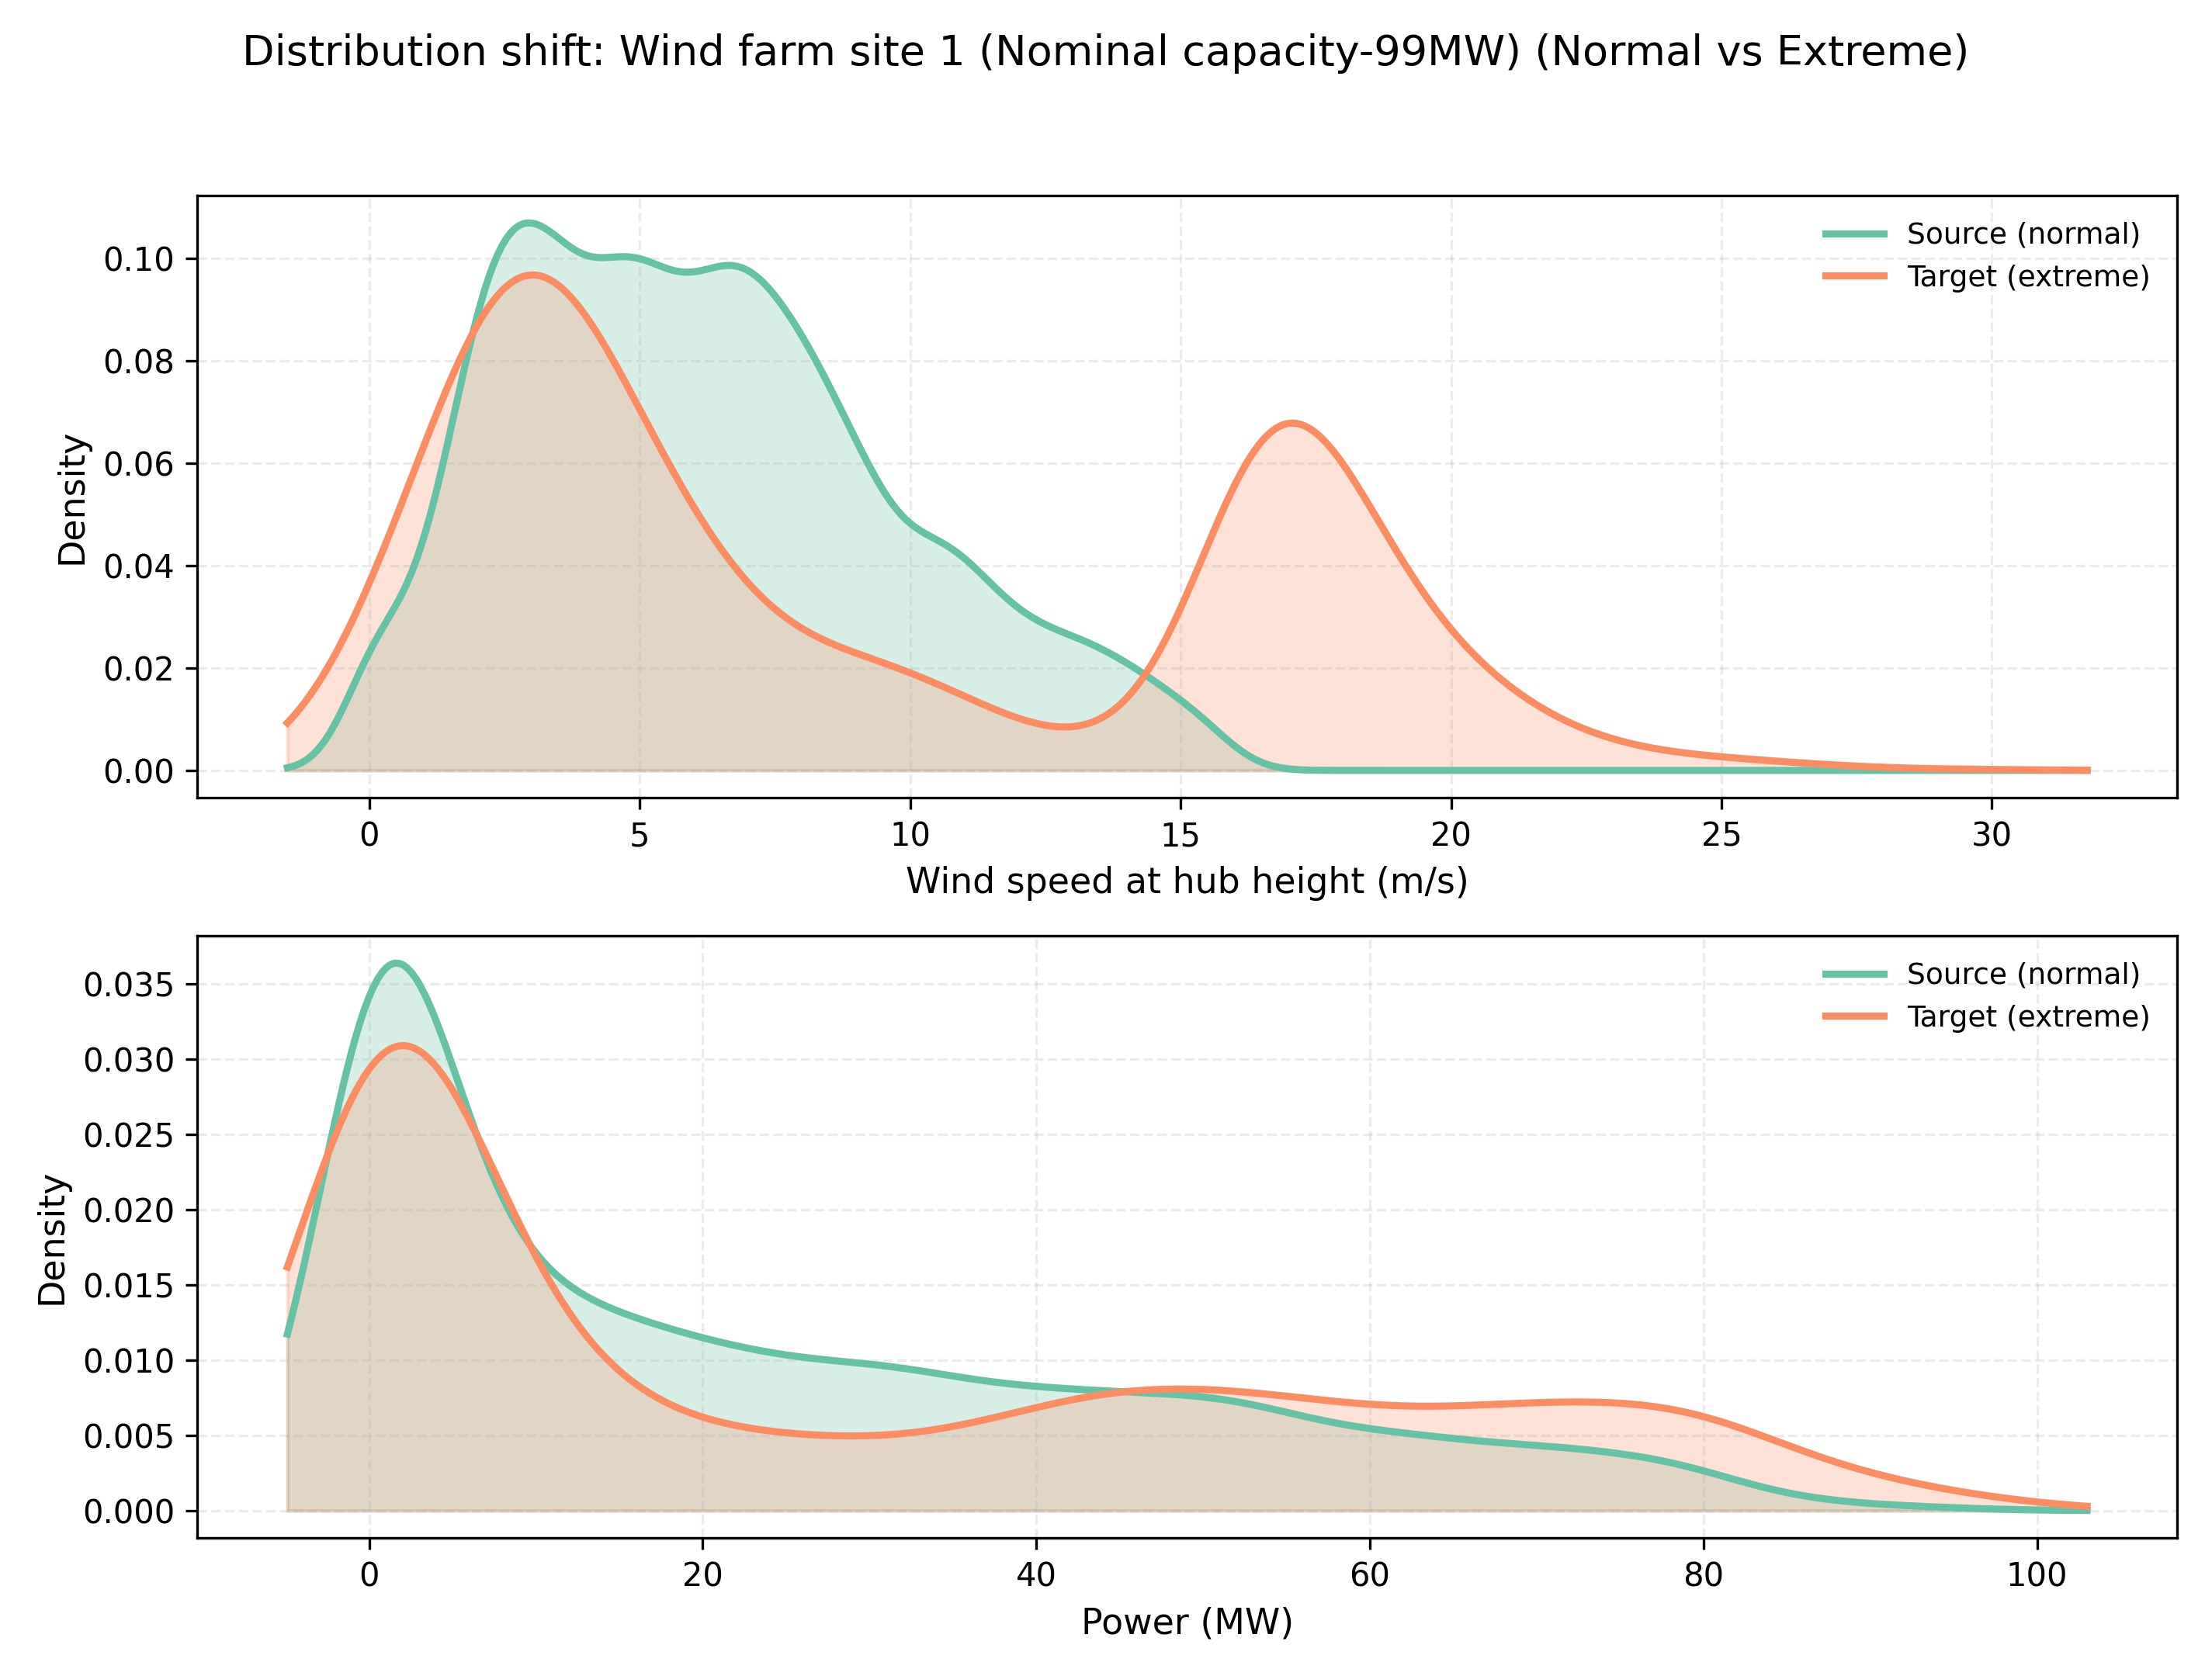
\includegraphics[width=0.46\textwidth]{experiment1/outputs/plots/farm1_domain_shift.jpg}
\hfill
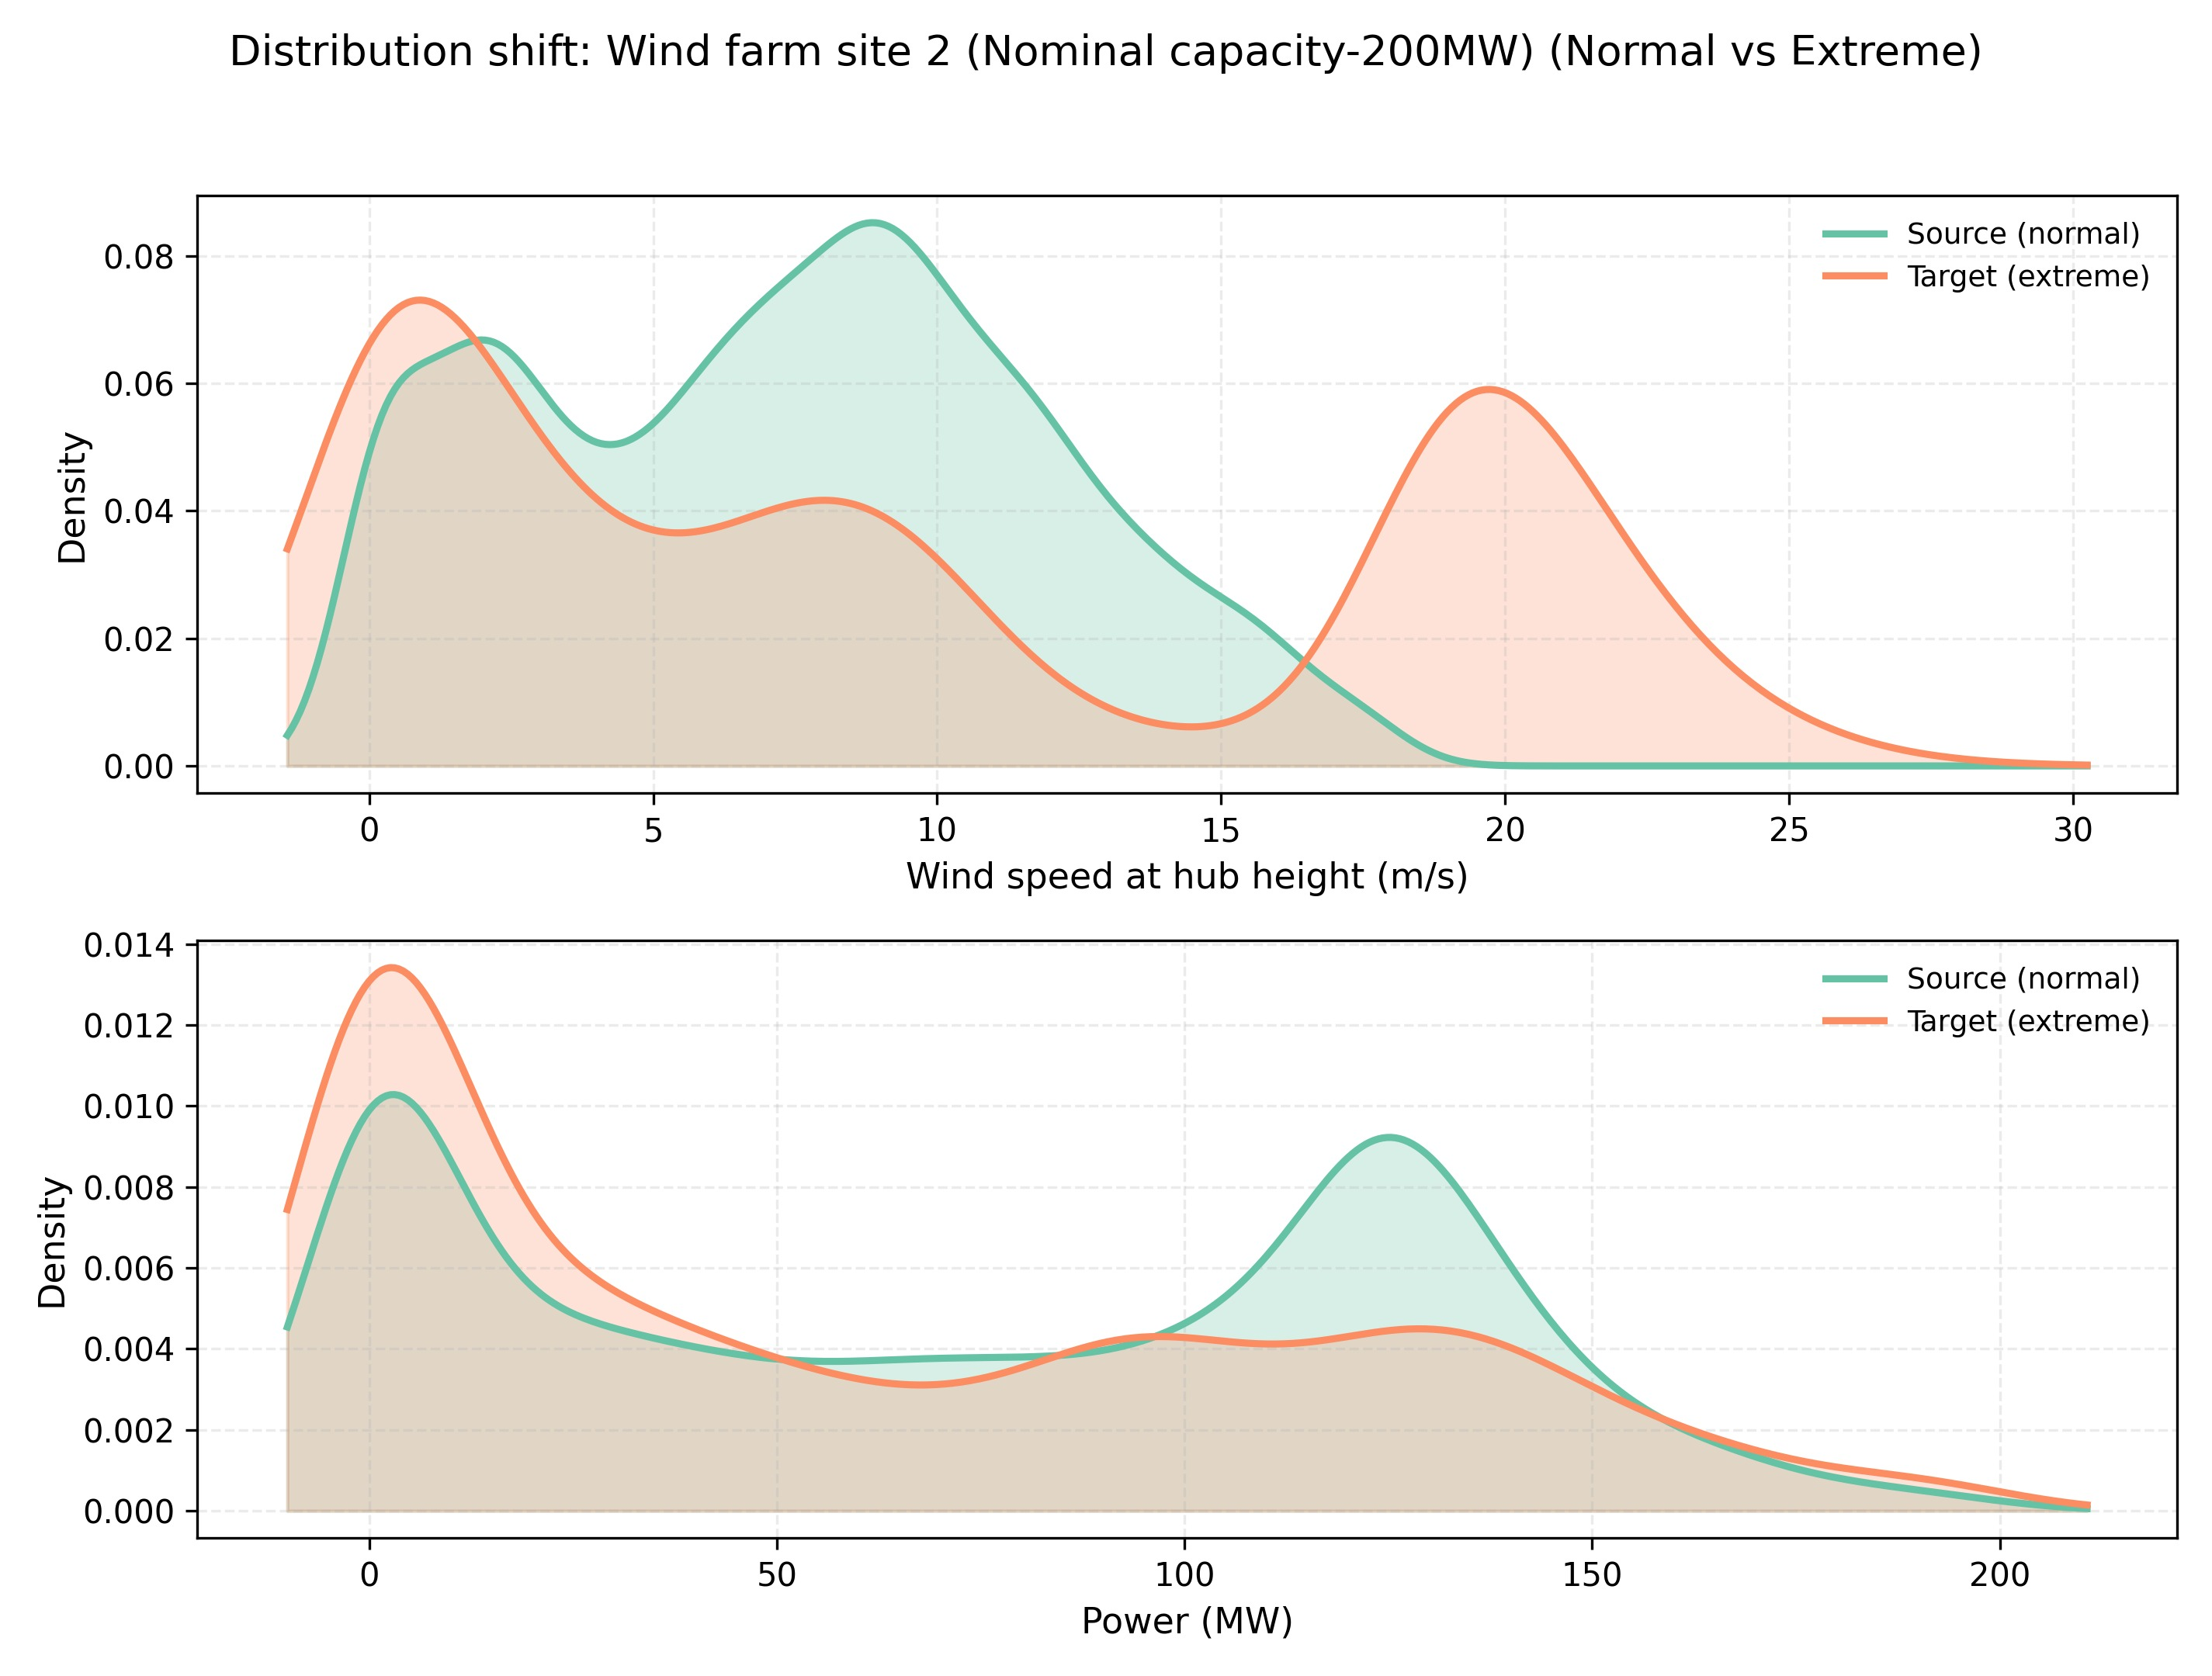
\includegraphics[width=0.46\textwidth]{experiment1/outputs/plots/farm0_domain_shift.jpg}

\vspace{0.12cm}
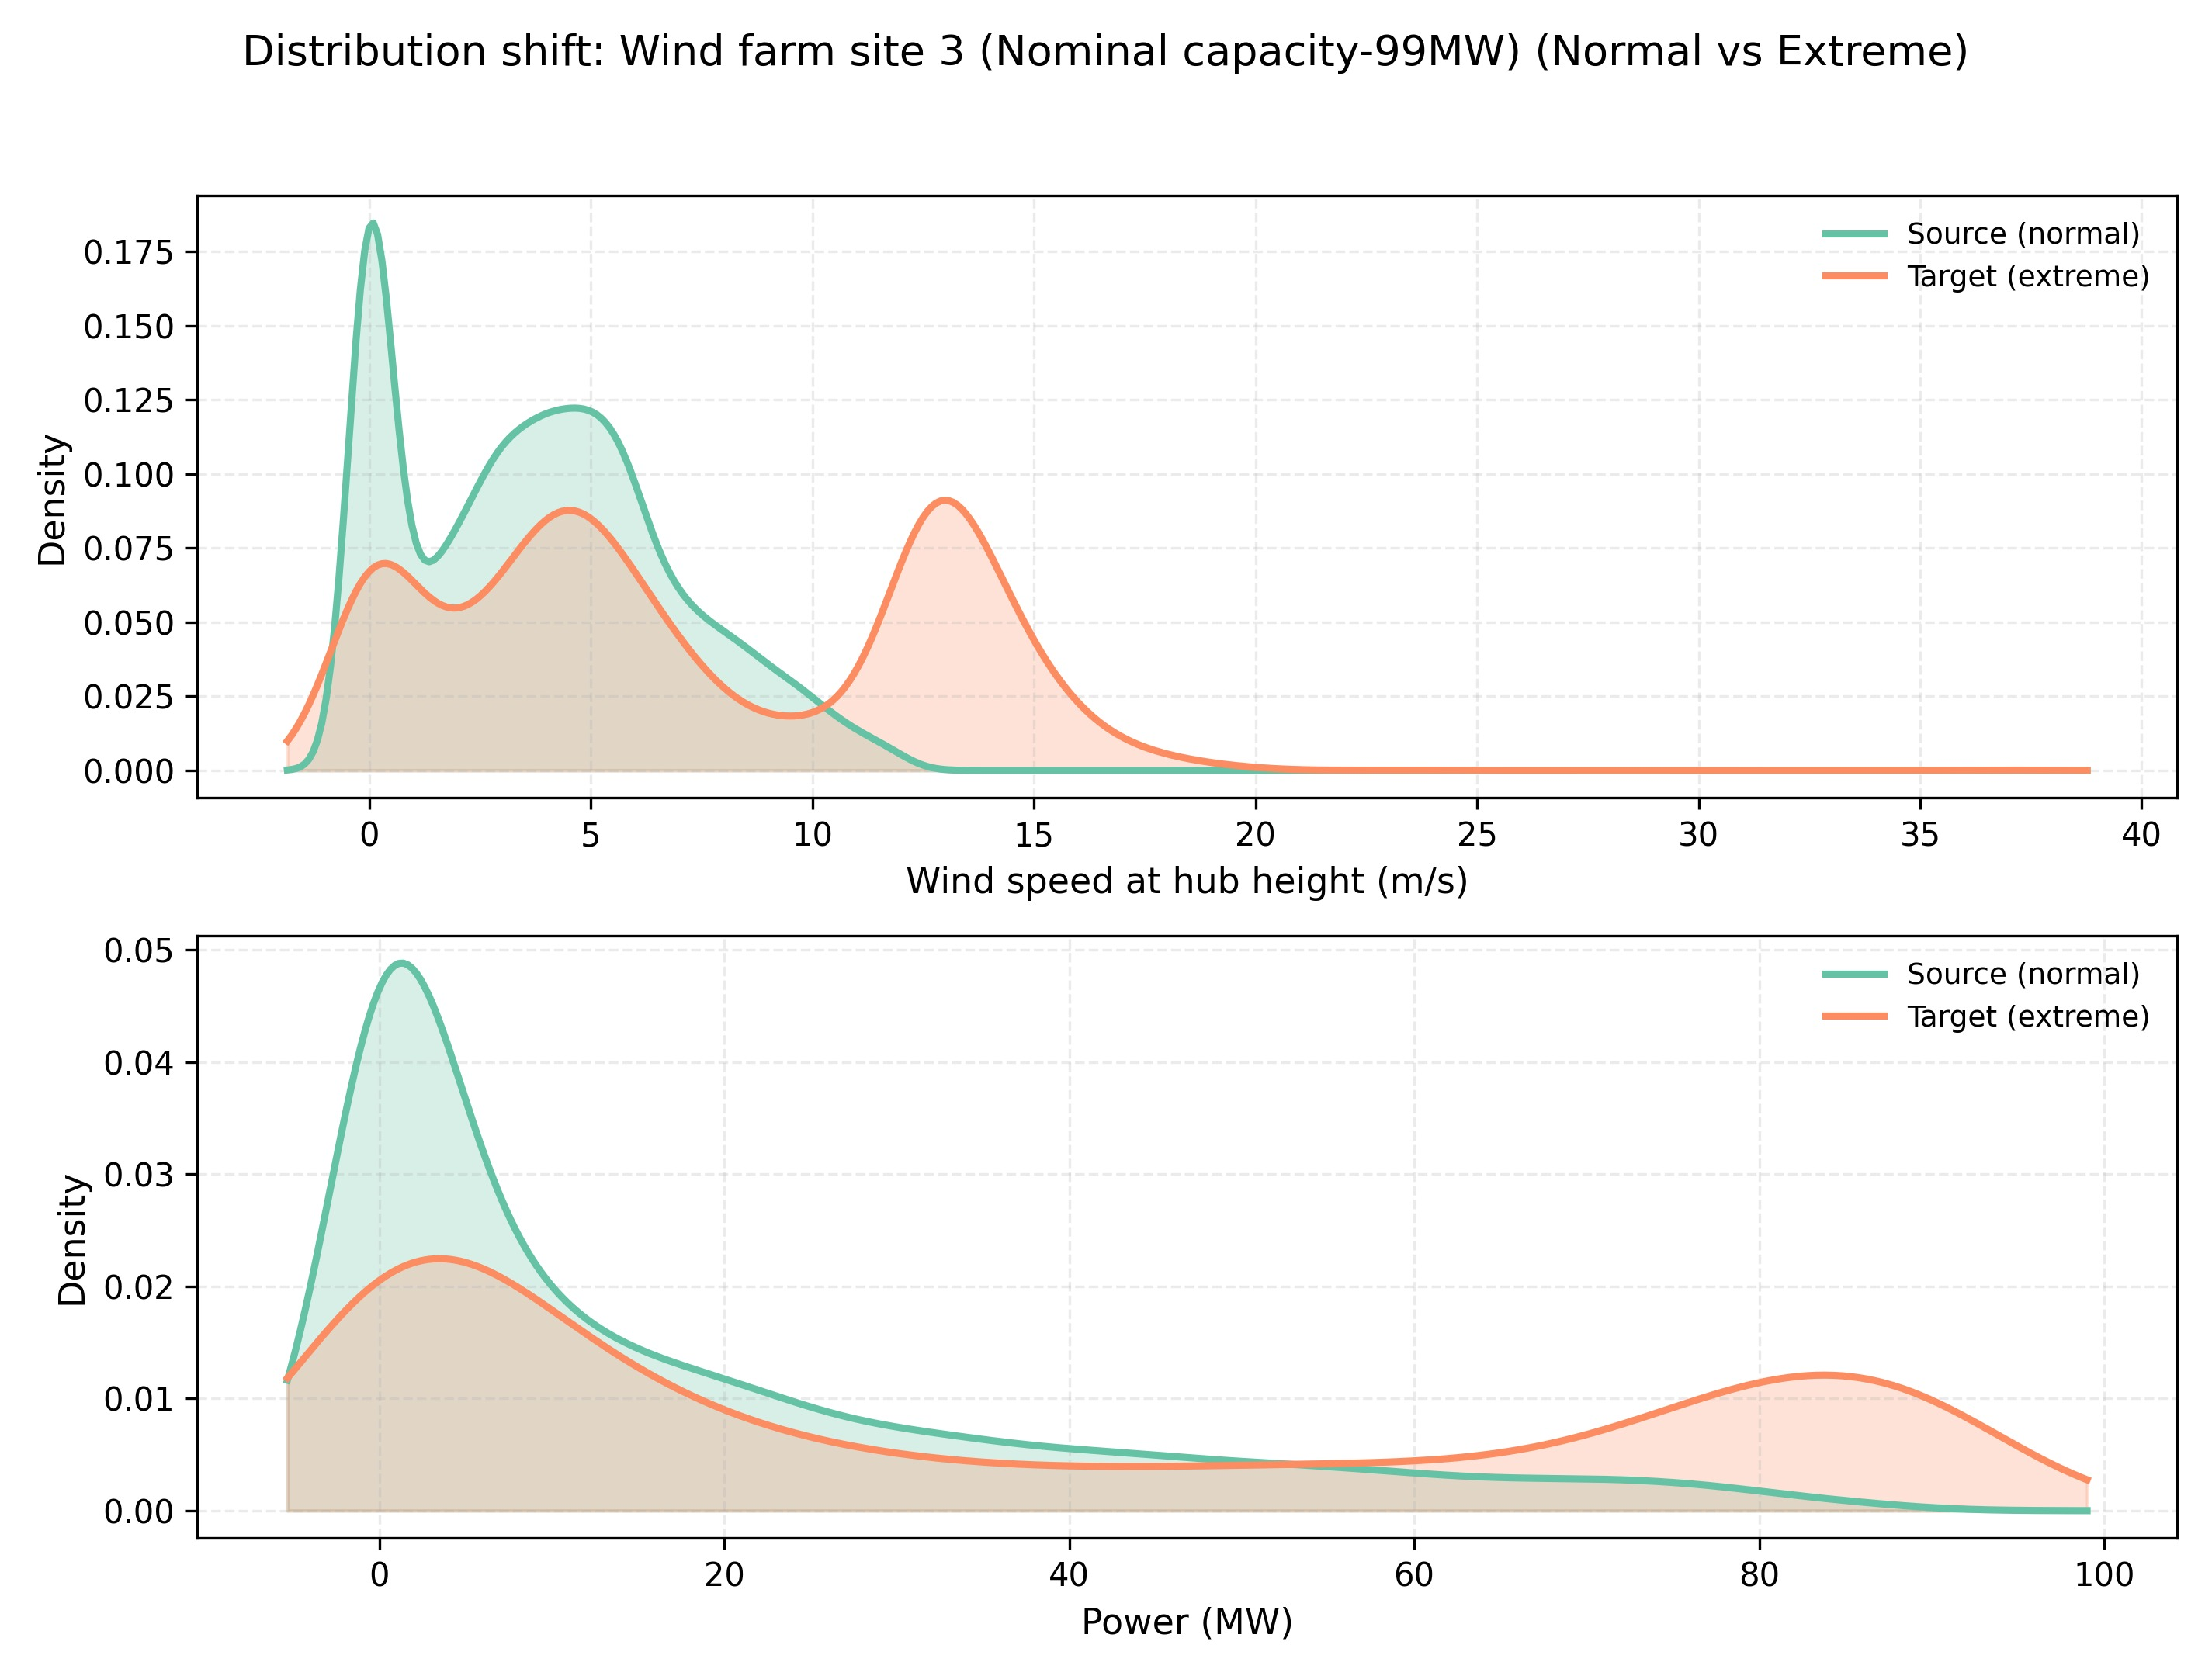
\includegraphics[width=0.46\textwidth]{experiment1/outputs/plots/farm2_domain_shift.jpg}
\hfill
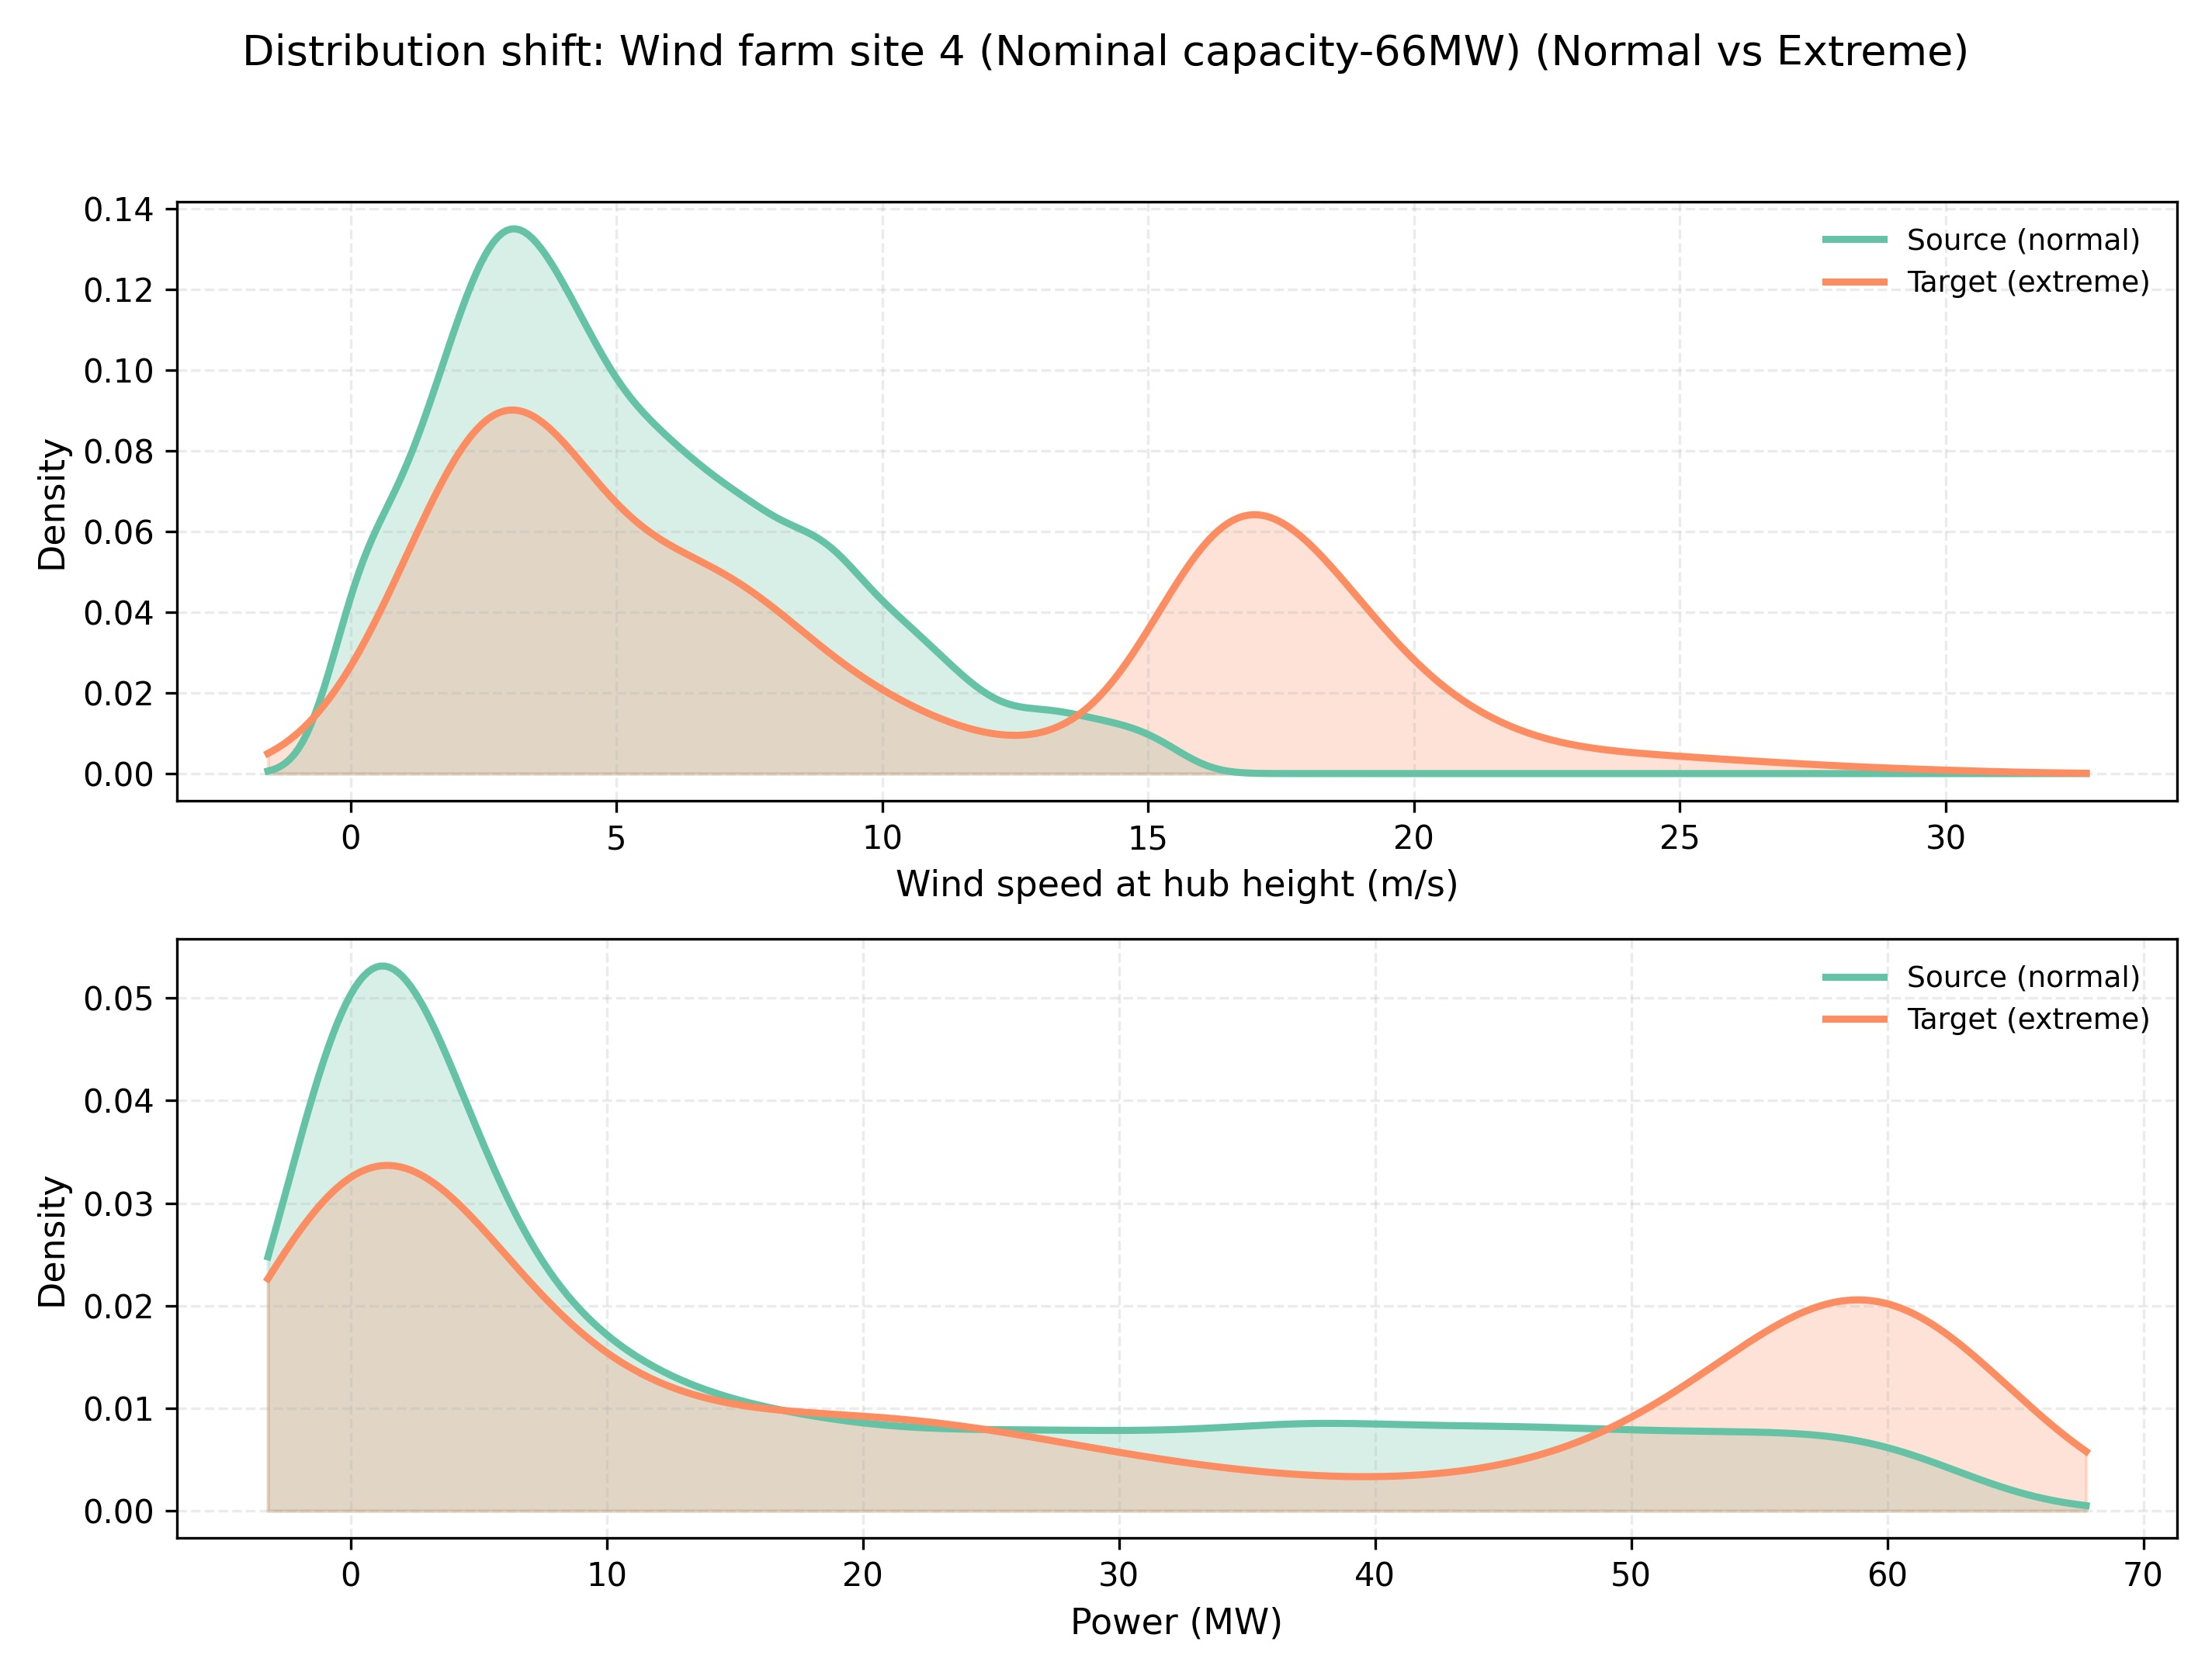
\includegraphics[width=0.46\textwidth]{experiment1/outputs/plots/farm4_domain_shift.jpg}

\vspace{0.12cm}
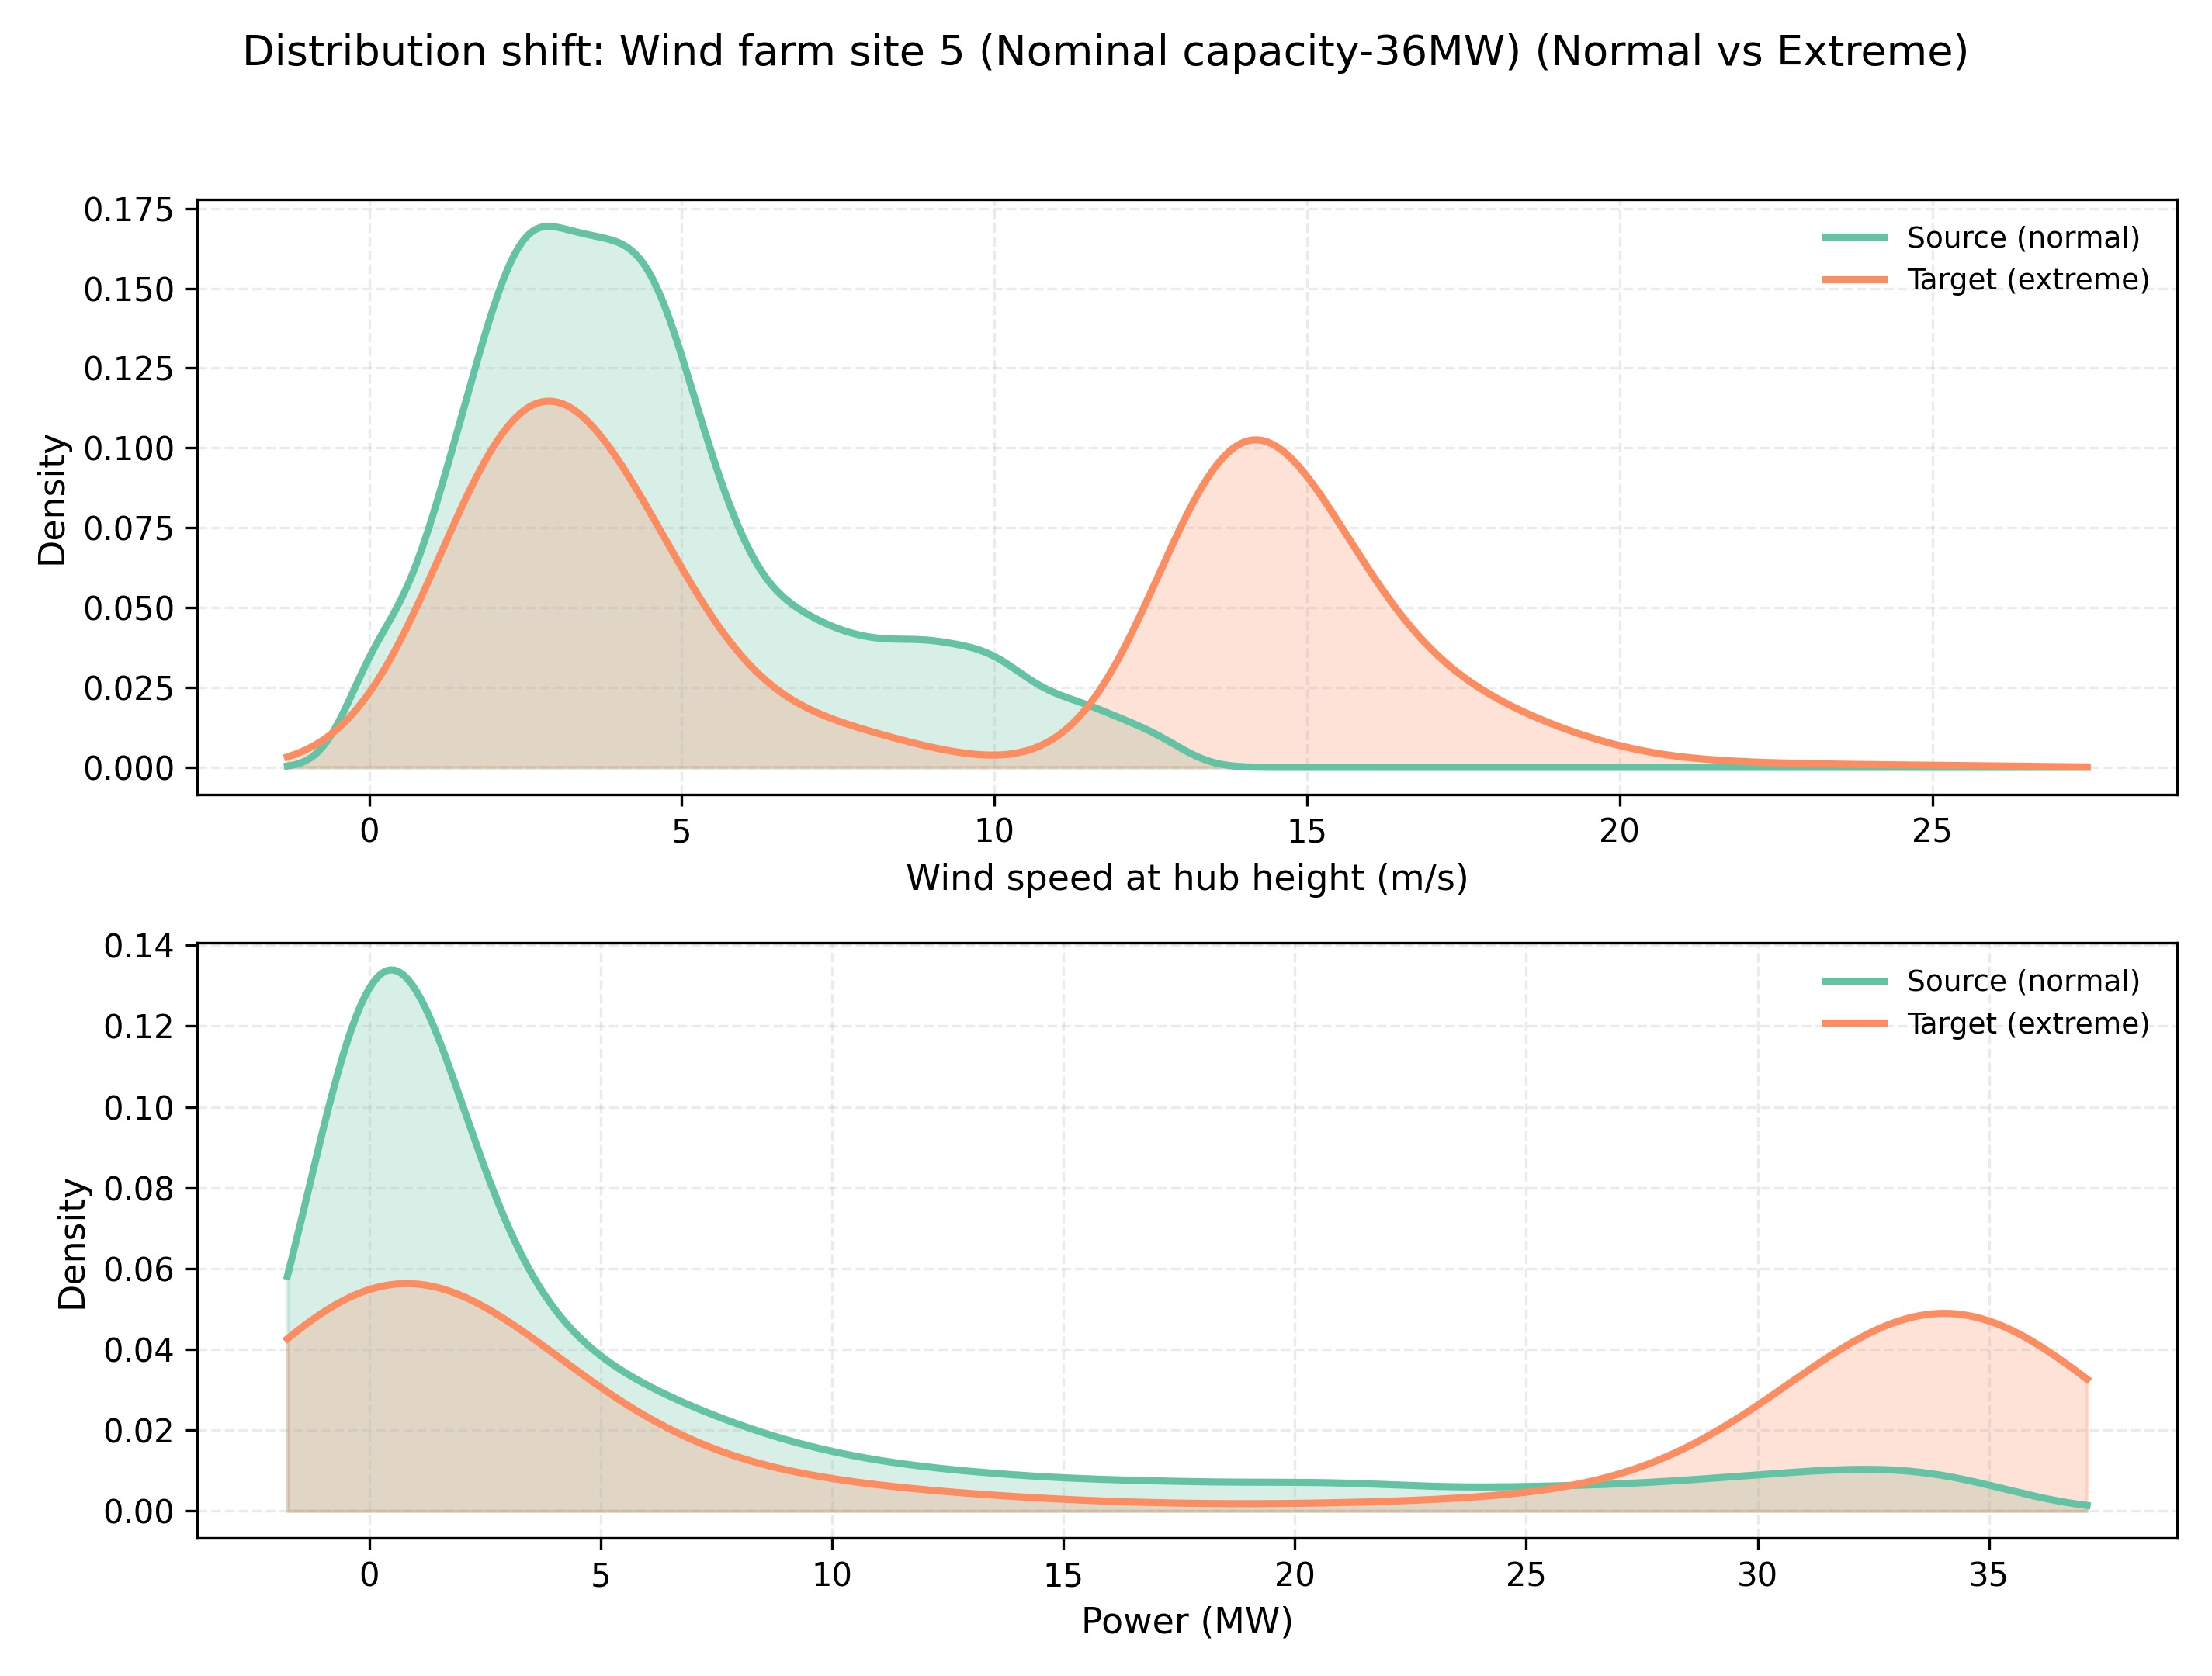
\includegraphics[width=0.46\textwidth]{experiment1/outputs/plots/farm5_domain_shift.jpg}
\hfill
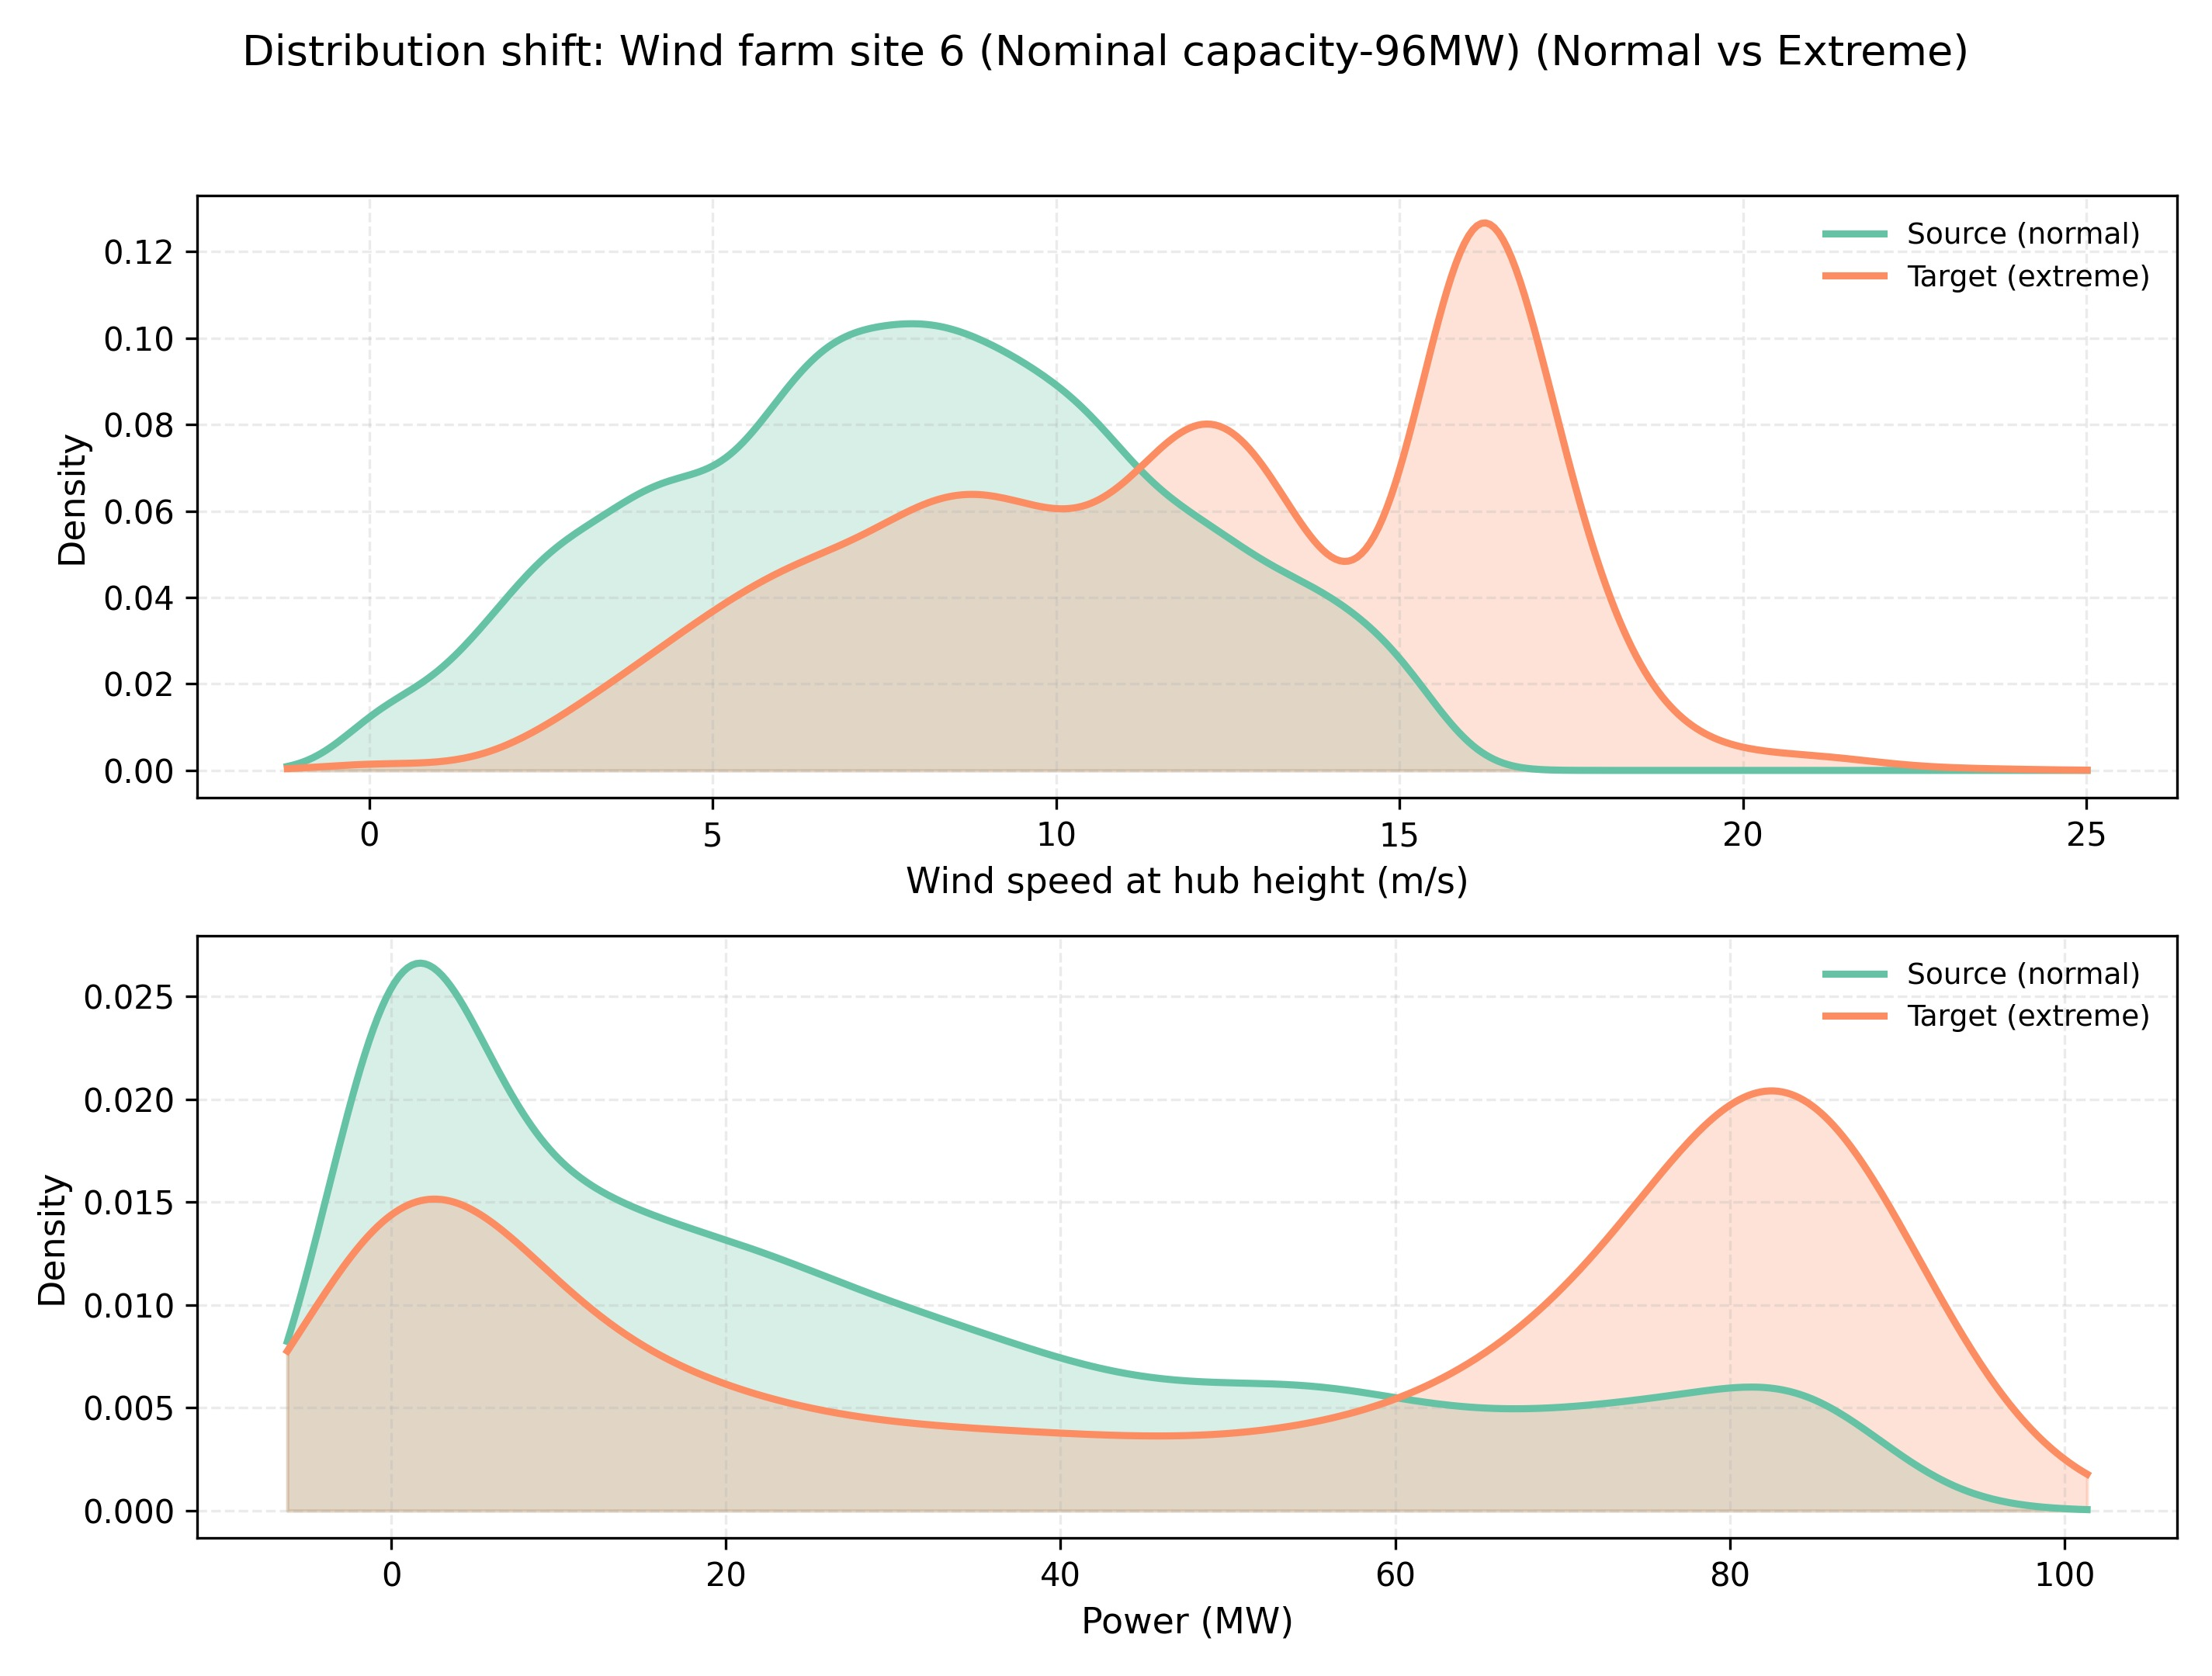
\includegraphics[width=0.46\textwidth]{experiment1/outputs/plots/farm3_domain_shift.jpg}
\captionof{figure}{Distribution shift visualization for all six wind farms. From left to right, top to bottom: Site~1 (99\,MW), Site~2 (200\,MW), Site~3 (99\,MW), Site~4 (66\,MW), Site~5 (36\,MW), and Site~6 (96\,MW). Each subplot shows kernel density estimates of wind speed (upper panel) and power output (lower panel) for the normal-operating (source) and extreme-event (target) domains. Site~6 exhibits the most severe domain shift in the power dimension.}
\label{fig:domain_shift}
\end{center}

%---------------- Experiment 2 --------------------%
\subsection{Experiment 2: Deterministic Point Prediction under Extreme Events}\label{sec:exp2}

The second experiment evaluates deterministic point prediction on Farm~6 and compares TL-QLDMR with nine baselines under the same data split and preprocessing protocol.

The data partition for Farm~6 is as follows:
\begin{itemize}
    \item \textbf{Source domain} (normal operation): 66{,}009 samples;
    \item \textbf{Target domain} (extreme-event domain): 4{,}143 samples.
\end{itemize}

We compare TL-QLDMR against nine baselines. The kernel-based baselines are SVR, LDMR, bounded-loss SVR (BLSSVR) \citep{fu2023bounded}, Harris hawks optimization SVR (HHO-SVR) \citep{houssein2025hho}, functional-iterative Lagrangian SVR (FLSVR) \citep{meena2025flsvr}, and associated-road-analysis SVR (ARA-SVR) \citep{duan2025ara}. The ensemble baselines are K-means clustering with gradient-boosted trees (KMeans-GBT) \citep{rizkallah2025kmeans}, random-forest wind power forecasting (RF-WPF) \citep{mustaffa2025rf}, and broad random-forest wind power forecasting (BRF-WPF) \citep{chen2025brf}.

\begin{table}[ht]
\centering
\caption{Deterministic point prediction results on the extreme-event test set of Farm~6. Best results are highlighted in bold (similarly hereinafter).}
\setlength{\tabcolsep}{3.5mm}
\begin{tabular}{lccc}
\toprule
Model & RMSE & MAE & $R^2$ \\
\midrule
LDMR & 10.692 & 6.327 & 0.9085 \\
BLSSVR        & 10.273 & 6.140 & 0.9155 \\
ARA-SVR       & 9.246 & 5.954 & 0.9316 \\
FLSVR         & 8.794 & 6.301 & 0.9381 \\
SVR  & 8.564 & 5.537 & 0.9413 \\
HHO-SVR       & 7.603 & 5.530 & 0.9537 \\
BRF-WPF       & 9.719 & 6.870 & 0.9244 \\
KMeans-GBT    & 9.620 & 6.695 & 0.9259 \\
RF-WPF        & 7.967 & 5.344 & 0.9492 \\
\textbf{TL-QLDMR (Ours)} & \textbf{7.478} & \textbf{5.248} & \textbf{0.9557} \\
\bottomrule
\end{tabular}
\label{tab:exp2_results}
\end{table}

\begin{figure}
\centering
\begin{minipage}[t]{0.49\linewidth}
\centering
(a) LDMR\par
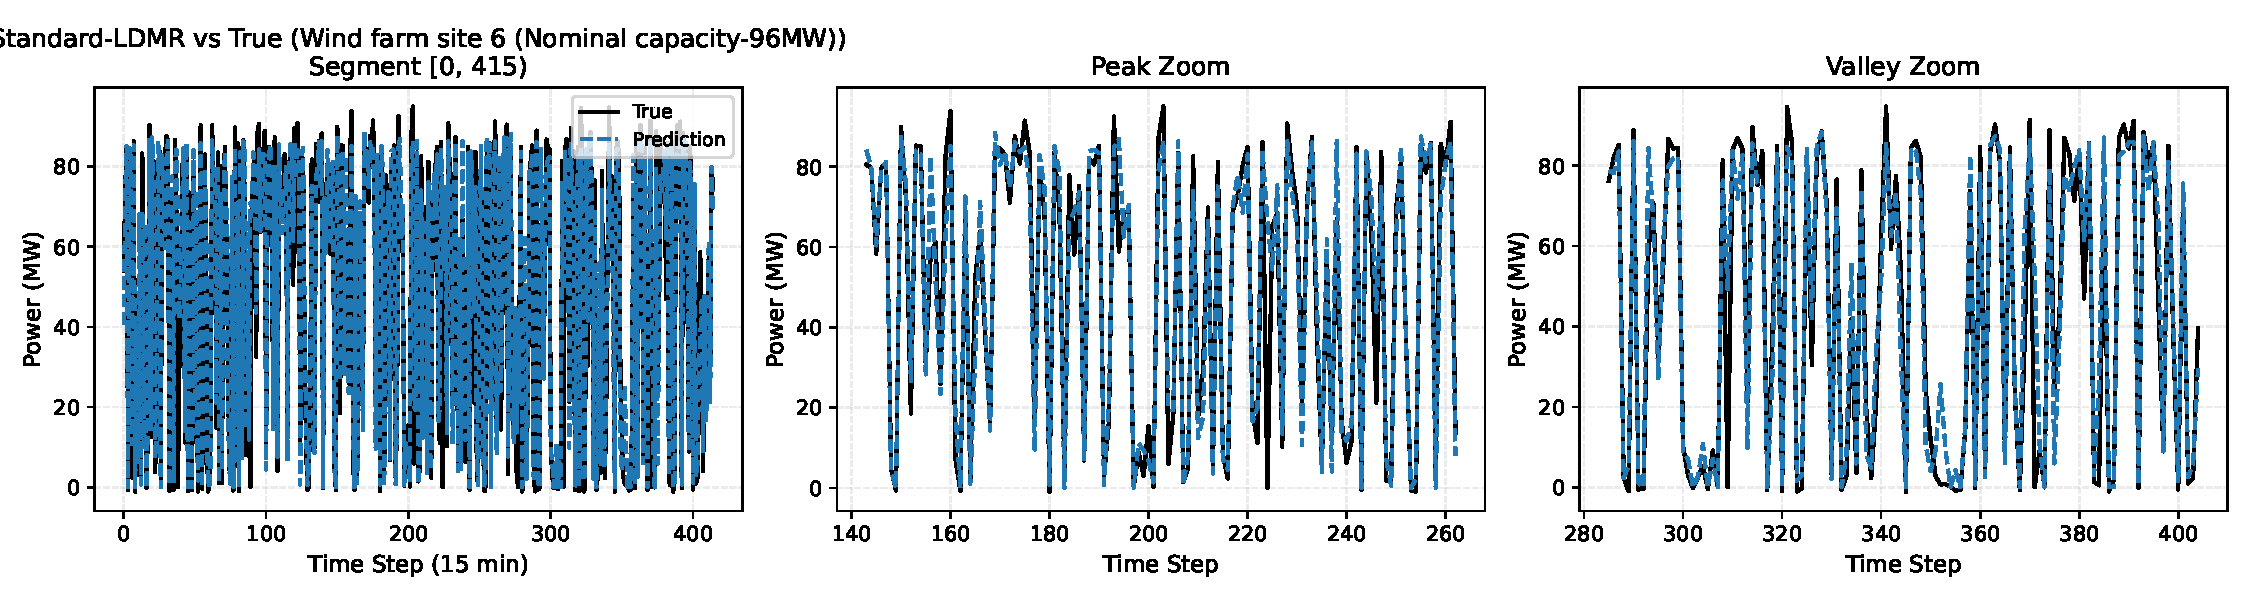
\includegraphics[width=\linewidth]{experiment2/plots_selected/farm3_Standard-LDMR.pdf}
\end{minipage}\hfill
\begin{minipage}[t]{0.49\linewidth}
\centering
(b) BLSSVR\par
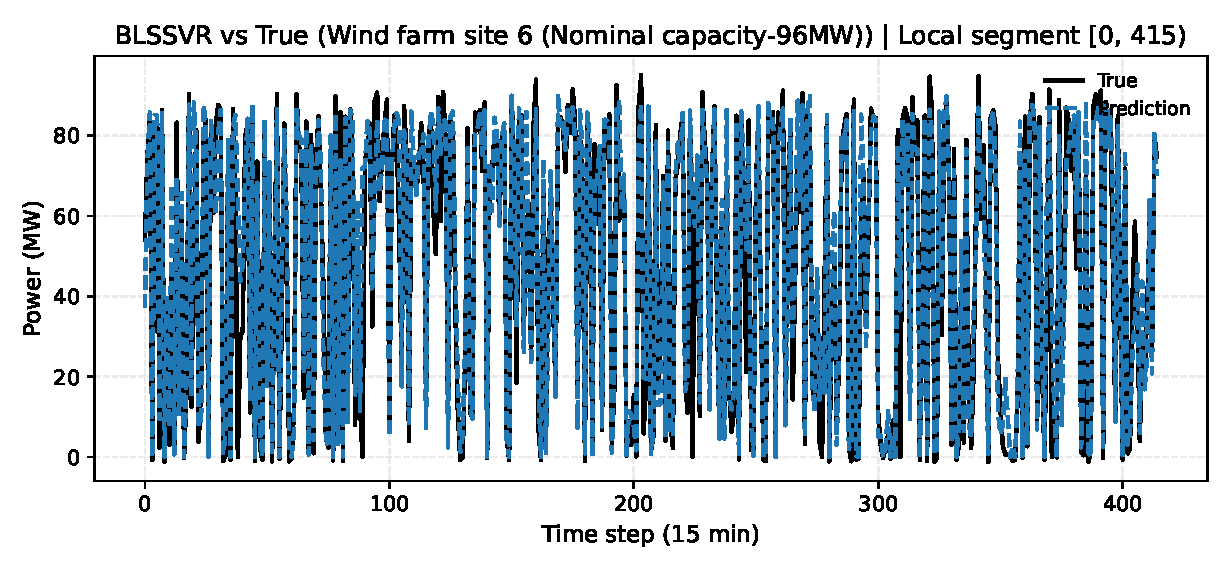
\includegraphics[width=\linewidth]{experiment2/plots_selected/farm3_BLSSVR.pdf}
\end{minipage}
\caption{Prediction comparison over selected temporal segments on the Farm~6 extreme-event test set (Part I).}
\label{fig:exp2_curves_a}
\end{figure}

\begin{figure}
\centering
\begin{minipage}[t]{0.49\linewidth}
\centering
(c) ARA-SVR\par
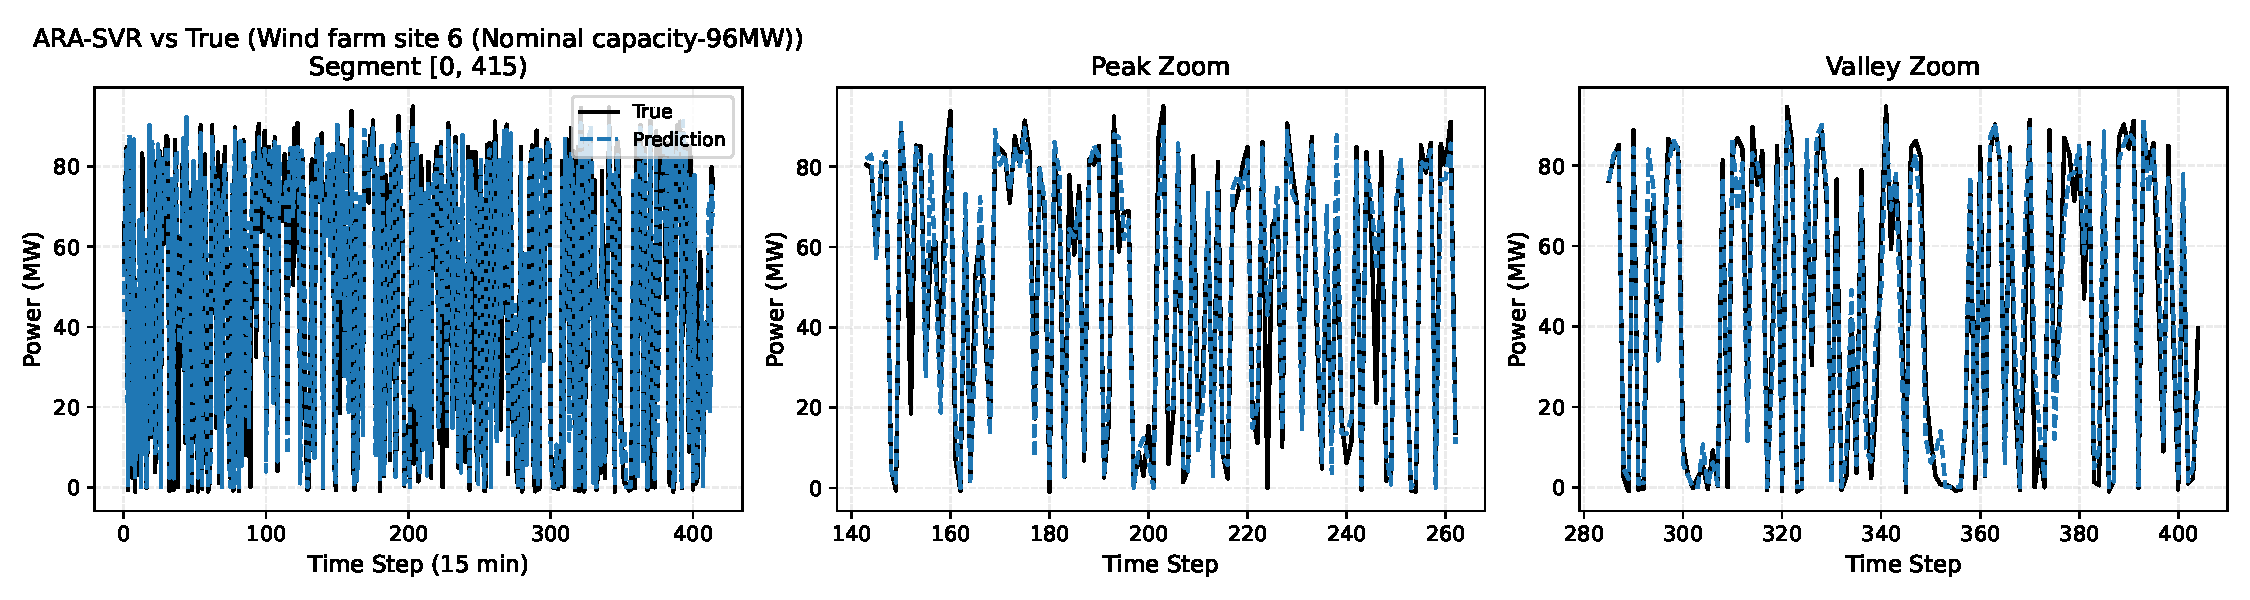
\includegraphics[width=\linewidth]{experiment2/plots_selected/farm3_ARA-SVR.pdf}
\end{minipage}\hfill
\begin{minipage}[t]{0.49\linewidth}
\centering
(d) FLSVR\par
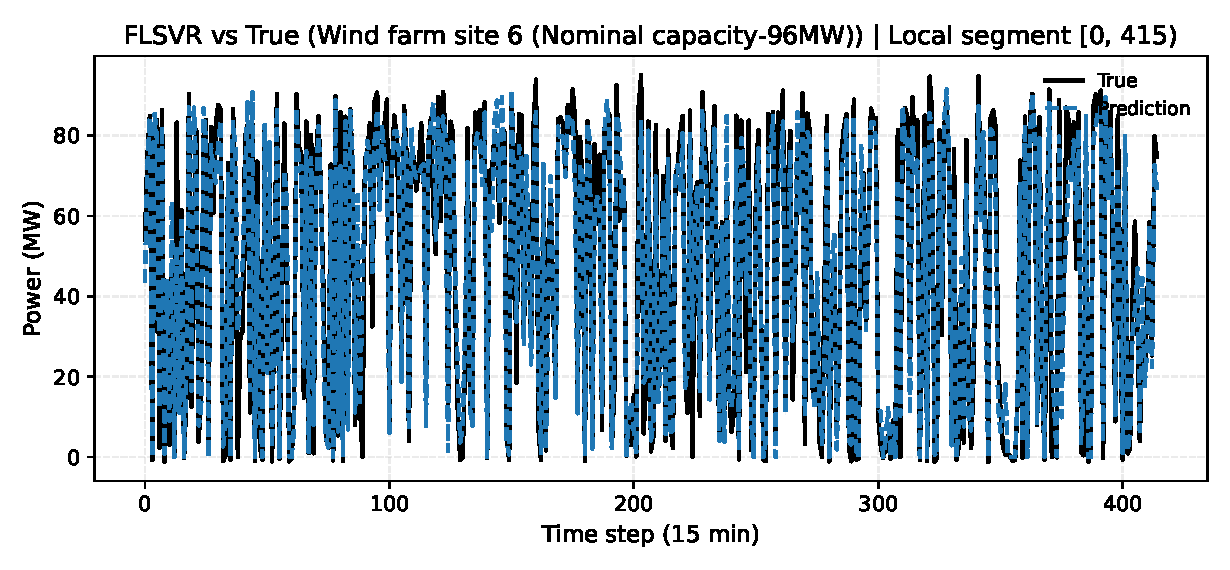
\includegraphics[width=\linewidth]{experiment2/plots_selected/farm3_FLSVR.pdf}
\end{minipage}
\caption{Prediction comparison over selected temporal segments on the Farm~6 extreme-event test set (Part II).}
\label{fig:exp2_curves_b}
\end{figure}

\begin{figure}
\centering
\begin{minipage}[t]{0.49\linewidth}
\centering
(e) SVR\par
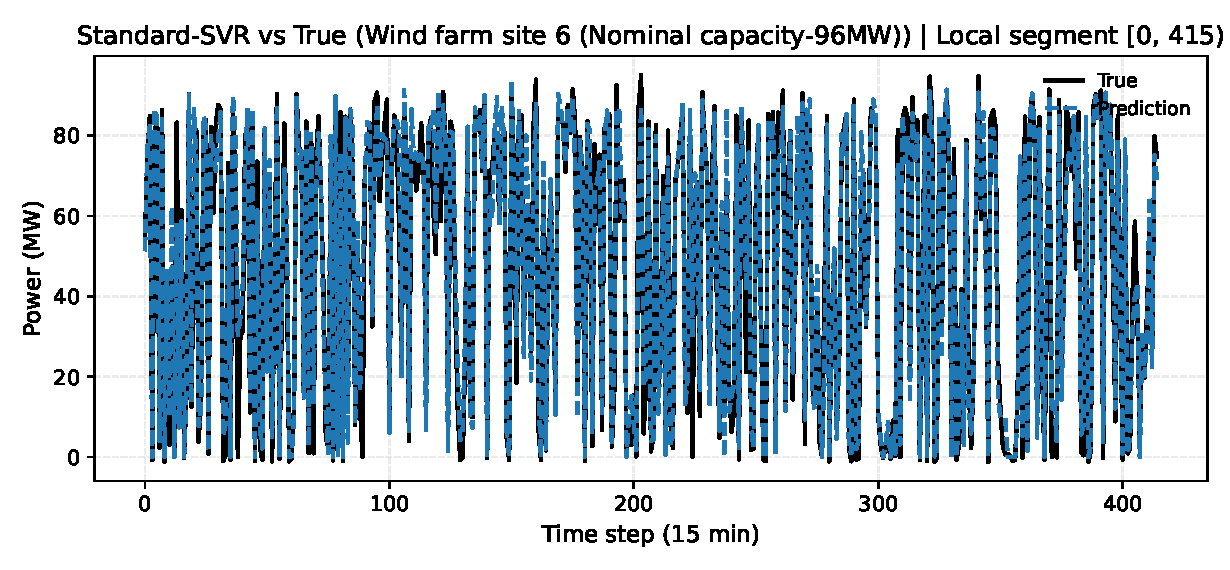
\includegraphics[width=\linewidth]{experiment2/plots_selected/farm3_Standard-SVR.pdf}
\end{minipage}\hfill
\begin{minipage}[t]{0.49\linewidth}
\centering
(f) HHO-SVR\par
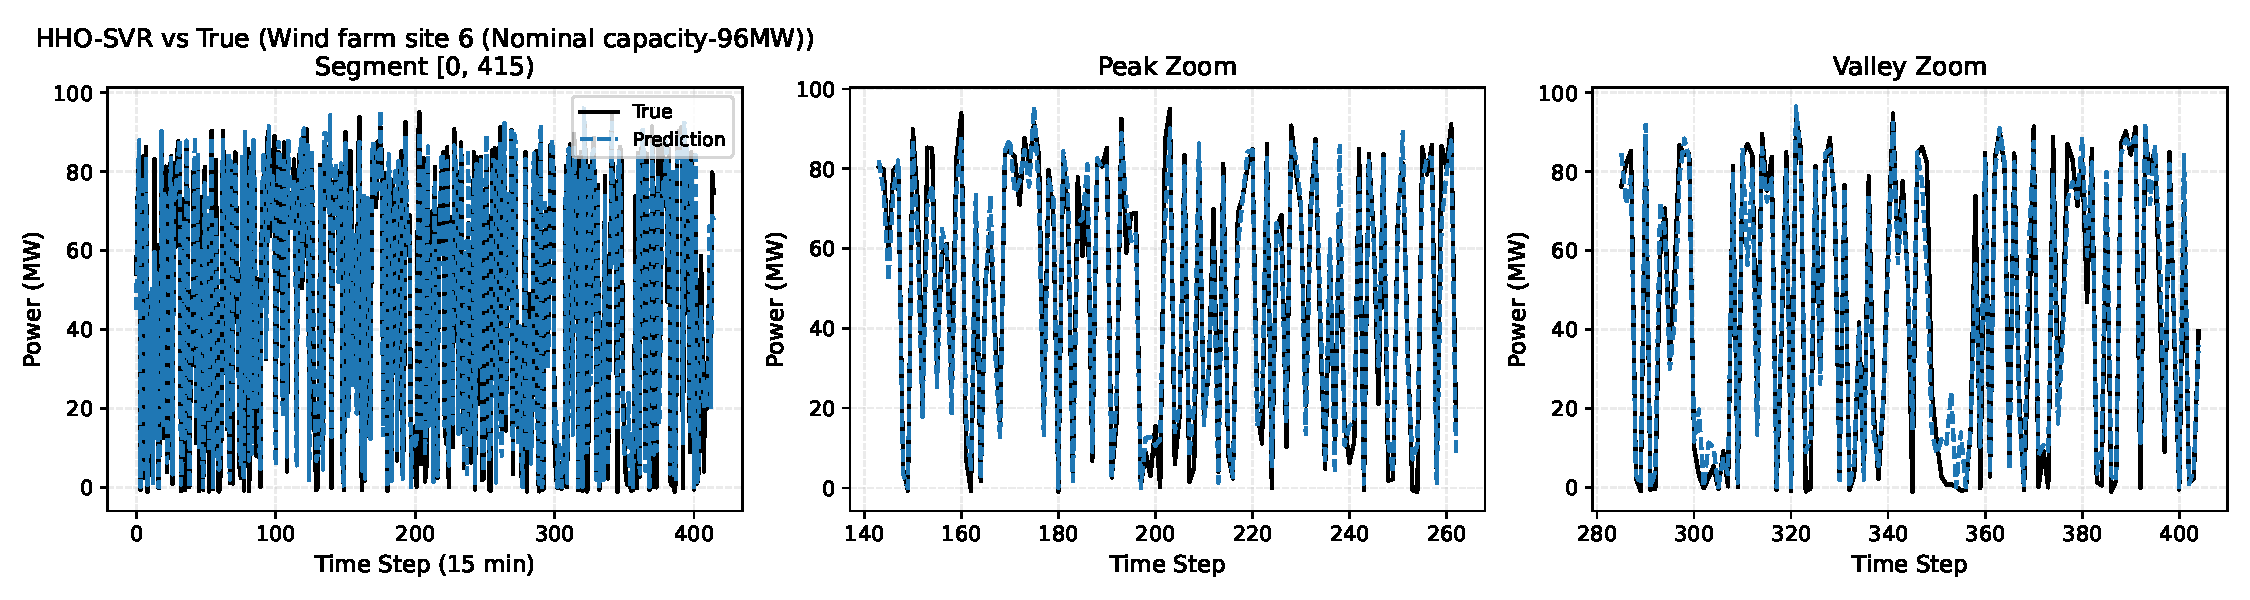
\includegraphics[width=\linewidth]{experiment2/plots_selected/farm3_HHO-SVR.pdf}
\end{minipage}
\caption{Prediction comparison over selected temporal segments on the Farm~6 extreme-event test set (Part III).}
\label{fig:exp2_curves_c}
\end{figure}

\begin{figure}
\centering
\begin{minipage}[t]{0.49\linewidth}
\centering
(g) BRF-WPF\par
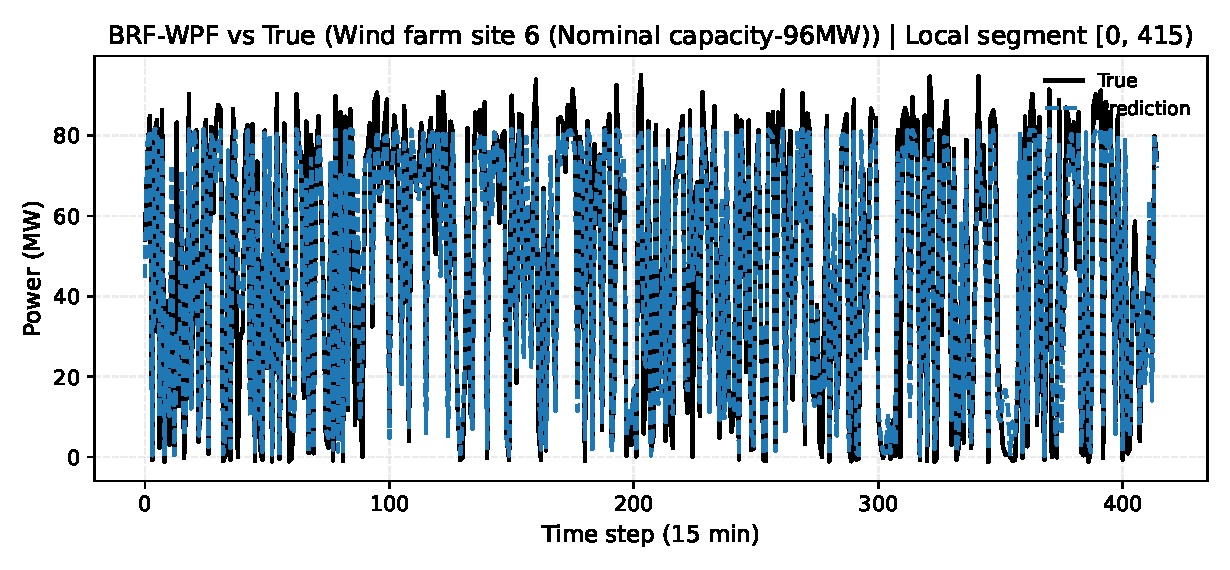
\includegraphics[width=\linewidth]{experiment2/plots_selected/farm3_BRF-WPF.pdf}
\end{minipage}\hfill
\begin{minipage}[t]{0.49\linewidth}
\centering
(h) KMeans-GBT\par
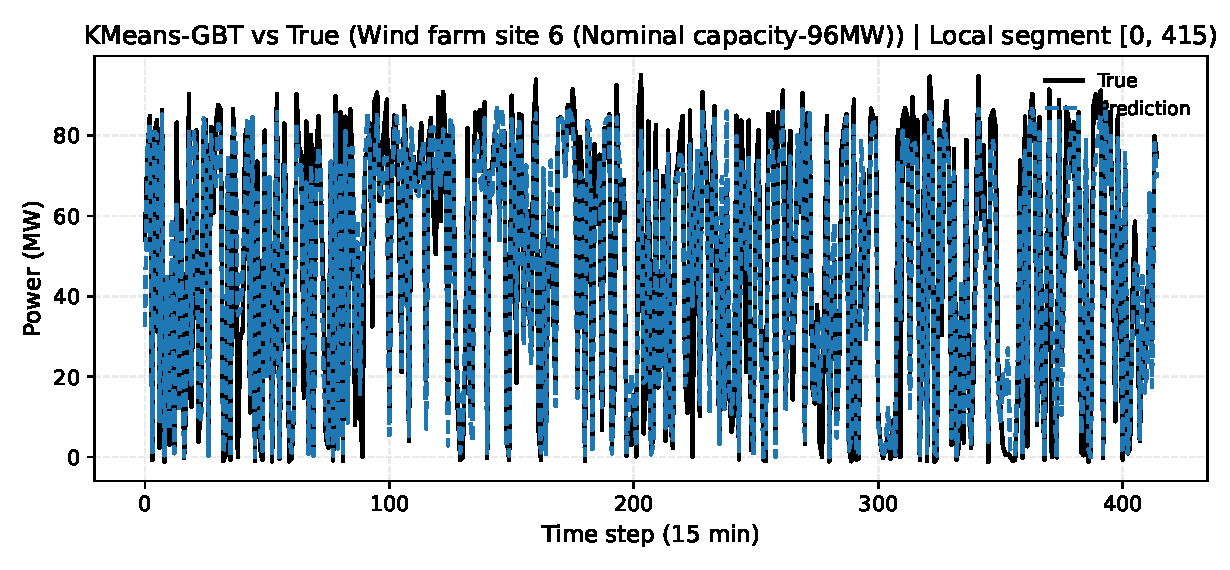
\includegraphics[width=\linewidth]{experiment2/plots_selected/farm3_KMeans-GBT.pdf}
\end{minipage}
\caption{Prediction comparison over selected temporal segments on the Farm~6 extreme-event test set (Part IV).}
\label{fig:exp2_curves_d}
\end{figure}

\begin{center}
\captionsetup{type=figure,hypcap=false}
\begin{minipage}[t]{0.47\linewidth}
\centering
(i) RF-WPF\par
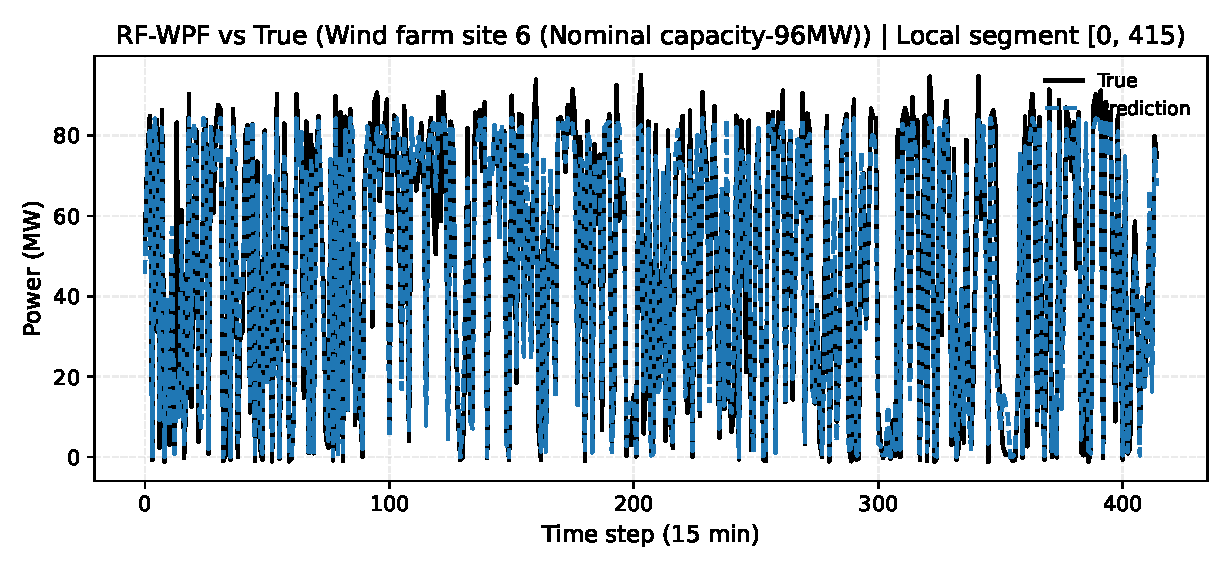
\includegraphics[width=0.96\linewidth]{experiment2/plots_selected/farm3_RF-WPF.pdf}
\end{minipage}\hfill
\begin{minipage}[t]{0.47\linewidth}
\centering
(j) TL-QLDMR\par
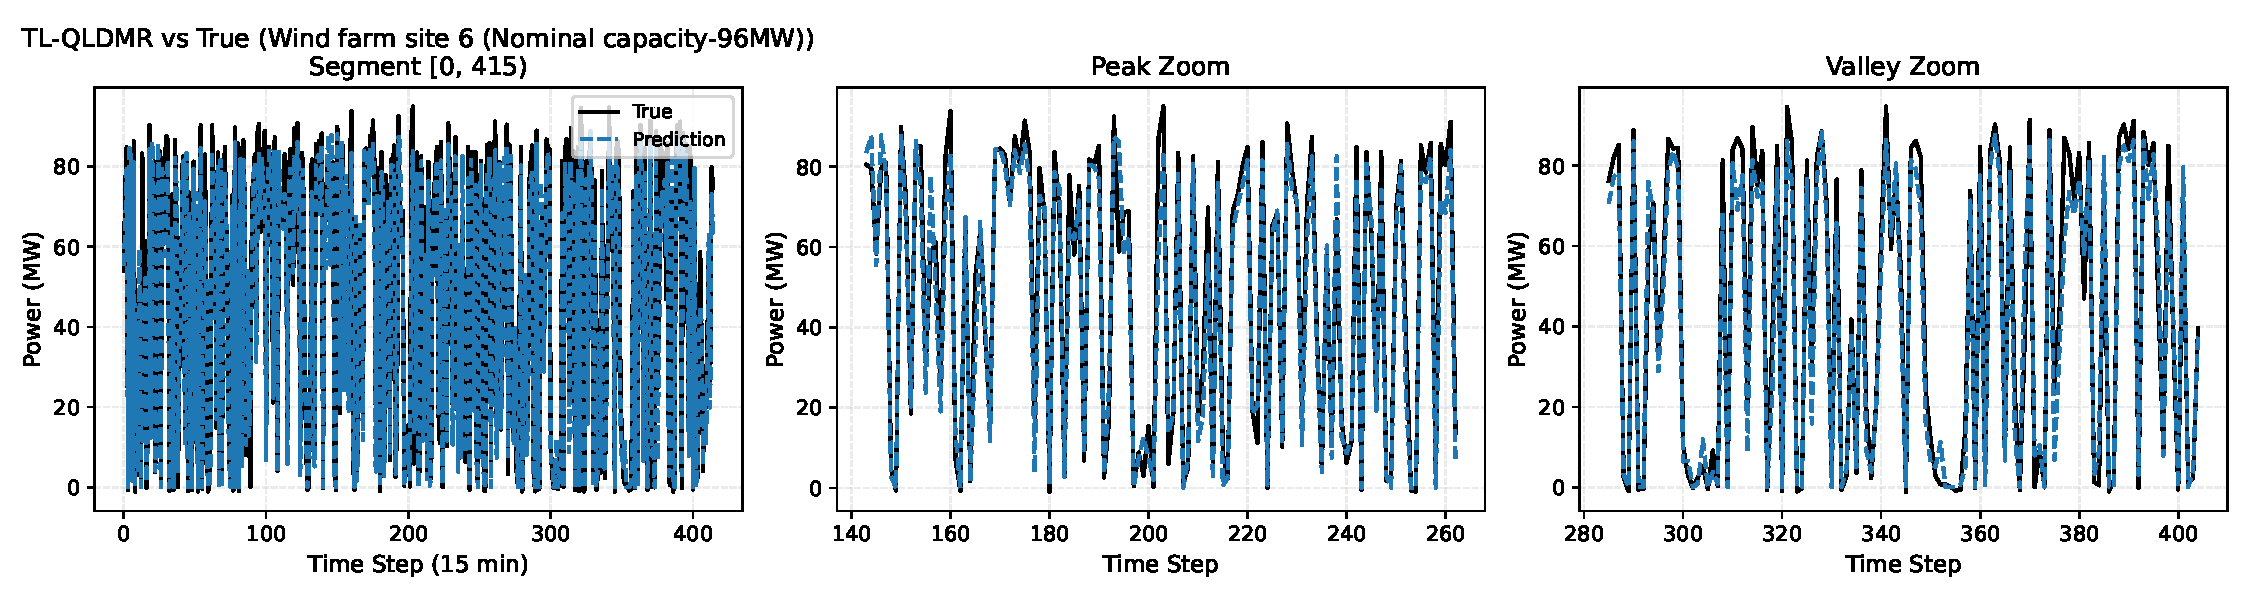
\includegraphics[width=0.96\linewidth]{experiment2/plots_selected/farm3_TL-QLDMR.pdf}
\end{minipage}
\captionof{figure}{Prediction comparison over selected temporal segments on the Farm~6 extreme-event test set (Part V).}
\label{fig:exp2_curves_e}
\end{center}

Table~\ref{tab:exp2_results} and Figs.~\ref{fig:exp2_curves_a}--\ref{fig:exp2_curves_e} jointly demonstrate that TL-QLDMR provides the most accurate and stable point forecasts on the Farm~6 extreme-event test set. LDMR exhibits the weakest performance among kernel methods (RMSE = 10.692, $R^2$ = 0.9085), confirming that symmetric variance regularization alone is insufficient in the cross-domain extreme-event setting. TL-QLDMR improves on the strongest non-transfer baselines: relative to HHO-SVR, it raises $R^2$ from 0.9537 to 0.9557 and reduces RMSE from 7.603 to 7.478; it also improves on RF-WPF (RMSE from 7.967 to 7.478). The segment-level evidence in Figs.~\ref{fig:exp2_curves_a}--\ref{fig:exp2_curves_e} confirms that TL-QLDMR tracks abrupt ramps and low-power transitions more closely than weaker baselines.

To assess the robustness of the models against measurement noise, which is prevalent in SCADA systems during extreme events, we evaluate the point prediction performance by injecting Gaussian noise into both the training and testing input features at signal-to-noise ratios (SNRs) of 60, 40, and 30\,dB.
The $R^2$ results under different noise levels are summarized in Table~\ref{tab:exp2_noise}.

\begin{table}[ht]
\centering
\caption{Model performance ($R^2$) under varying SNR on the Farm~6 extreme-event test set.}
\setlength{\tabcolsep}{3.5mm}
\begin{tabular}{lccc}
\toprule
Model & SNR = 30 dB & SNR = 40 dB & SNR = 60 dB \\
\midrule
LDMR & 0.9084 & 0.9080 & 0.9084 \\
BLSSVR        & 0.9121 & 0.9146 & 0.9154 \\
ARA-SVR       & 0.9311 & 0.9316 & 0.9316 \\
FLSVR         & 0.9380 & 0.9381 & 0.9381 \\
SVR  & 0.9409 & 0.9414 & 0.9413 \\
HHO-SVR       & 0.9442 & 0.9438 & 0.9437 \\
BRF-WPF       & 0.9177 & 0.9250 & 0.9253 \\
KMeans-GBT    & 0.9209 & 0.9230 & 0.9262 \\
RF-WPF        & 0.9471 & 0.9485 & 0.9469 \\
\textbf{TL-QLDMR (Ours)} & \textbf{0.9584} & \textbf{0.9560} & \textbf{0.9603} \\
\bottomrule
\end{tabular}
\label{tab:exp2_noise}
\end{table}

TL-QLDMR consistently maintains the highest $R^2$ across all noise levels (0.9584, 0.9560, and 0.9603 at SNR = 30, 40, and 60\,dB). The strongest baseline under noisy inputs is HHO-SVR, but it remains below TL-QLDMR at all settings. The transfer learning framework, reinforced by asymmetric variance regularization, effectively mitigates overfitting to noisy target samples and demonstrates the strongest noise resilience among all comparative models.

%---------------- Experiment 3 --------------------%
\subsection{Experiment 3: Probabilistic Interval Prediction under Extreme Events}\label{sec:exp3}

The third experiment extends evaluation from point prediction to probabilistic interval forecasting. The objective is to verify whether TL-QLDMR can achieve reliable 95\% prediction intervals while keeping interval width sufficiently sharp under extreme-event volatility.

The interval prediction baselines include SVQR, twin support vector quantile regression (TSVQR) \citep{tsvqr2023}, a robust truncated-pinball SVQR baseline (UQSVM-SSVQR) \citep{wang2024ssvqr}, nonlinear feature selection SVQR (NFS-SVQR) \citep{ye2025nfs}, $\nu$-support vector regression with conformalized intervals (NuSVR-CI) \citep{romano2019cqr}, robust low-rank multiple kernel learning (RLMKL) \citep{jiang2021rlmkl}, a hybrid deep-learning interval model (HybridDL-Interval) \citep{hybriddl2025}, an attention-based recurrent neural network interval model (AMQRNN) \citep{amqrnn2025}, quantile gradient boosted regression (QGBR) \citep{hu2025ncqgbr}, and conformalized quantile regression multilayer perceptron (CQR-MLP) \citep{hu2025nescqr}.

Table~\ref{tab:exp3_results} presents the interval prediction results on the extreme-event test set of Farm~6 at the 95\% confidence level ($\alpha = 0.05$).

\begin{table*}[ht]
\centering
\caption{Interval prediction results on the extreme-event test set of Farm~6 at 95\% confidence level ($\alpha = 0.05$).}
\setlength{\tabcolsep}{4mm}
\begin{tabular}{lccccc}
\toprule
Model & PICP & MPIW & PINAW & CWC & Winkler \\
\midrule
NuSVR-CI            & 0.843 & \textbf{19.970} & \textbf{0.208} & 0.285 & 54.603 \\
HybridDL-Interval   & 0.954 & 31.645 & 0.329 & 0.329 & 60.224 \\
RLMKL               & 0.957 & 31.804 & 0.331 & 0.331 & 39.275 \\
TSVQR               & 0.889 & 24.592 & 0.256 & 0.342 & 48.178 \\
SVQR       & \textbf{0.959} & 34.342 & 0.357 & 0.357 & 42.067 \\
QGBR                & 0.949 & 31.715 & 0.330 & 0.429 & 37.643 \\
CQR-MLP             & 0.942 & 31.750 & 0.330 & 0.431 & 46.772 \\
AMQRNN              & 0.940 & 32.432 & 0.337 & 0.441 & 66.874 \\
NFS-SVQR            & 0.913 & 68.359 & 0.711 & 0.941 & 76.997 \\
UQSVM-SSVQR         & 0.928 & 81.710 & 0.850 & 1.117 & 85.162 \\
\textbf{TL-QLDMR (Ours)} & \textbf{0.959} & 25.791 & 0.268 & \textbf{0.268} & \textbf{34.506} \\
\bottomrule
\end{tabular}
\label{tab:exp3_results}
\end{table*}

TL-QLDMR reaches the nominal 95\% coverage target (PICP = 0.959) while obtaining the best composite quality (CWC = 0.268) and the best Winkler score (34.506). SVQR achieves the same coverage but produces substantially wider intervals (PINAW = 0.357 vs. 0.268). RLMKL provides a stronger robust-kernel baseline than conventional SVQR variants (Winkler = 39.275), but TL-QLDMR still achieves materially sharper and better-calibrated intervals. NuSVR-CI and TSVQR produce narrow intervals but severe under-coverage (PICP = 0.843 and 0.889), whereas deep learning baselines require wider intervals to approach acceptable coverage.

To assess interval robustness under sensor perturbation, Gaussian noise is injected into test inputs at SNR $\in \{60,40,30\}$ dB.
Table~\ref{tab:exp3_noise} reports the full set of interval metrics under this noisy-test protocol.

\FloatBarrier

\begin{table*}[ht]
\centering
\caption{Interval prediction results under varying SNR on the extreme-event test set of Farm~6 at 95\% confidence level ($\alpha = 0.05$).}
\setlength{\tabcolsep}{3.0mm}
\begin{tabular}{llccccc}
\toprule
Model & SNR (dB) & PICP & MPIW & PINAW & CWC & Winkler \\
\midrule
\multirow{3}{*}{NuSVR-CI}
  & 30 & 0.8386 & \textbf{19.970} & \textbf{0.2077} & 0.2856 & 54.922 \\
  & 40 & 0.8361 & \textbf{19.970} & \textbf{0.2077} & 0.2860 & 54.623 \\
  & 60 & 0.8434 & \textbf{19.970} & \textbf{0.2077} & 0.2849 & 54.588 \\
\multirow{3}{*}{HybridDL-Interval}
  & 30 & 0.9422 & 32.304 & 0.3360 & 0.4384 & 53.462 \\
  & 40 & 0.9422 & 32.307 & 0.3361 & 0.4385 & 53.420 \\
  & 60 & 0.9422 & 32.306 & 0.3361 & 0.4385 & 53.408 \\
\multirow{3}{*}{RLMKL}
  & 30 & 0.9494 & 30.161 & 0.3138 & 0.4080 & 39.063 \\
  & 40 & 0.9494 & 30.101 & 0.3131 & 0.4072 & 39.235 \\
  & 60 & 0.9494 & 30.095 & 0.3131 & 0.4071 & 39.200 \\
\multirow{3}{*}{TSVQR}
  & 30 & 0.8892 & 24.570 & 0.2556 & 0.3422 & 48.306 \\
  & 40 & 0.8892 & 24.588 & 0.2558 & 0.3424 & 48.140 \\
  & 60 & 0.8892 & 24.592 & 0.2558 & 0.3425 & 48.169 \\
\multirow{3}{*}{SVQR}
  & 30 & 0.9446 & 29.704 & 0.3090 & 0.4027 & 41.541 \\
  & 40 & 0.9422 & 29.725 & 0.3092 & 0.4034 & 41.429 \\
  & 60 & 0.9446 & 29.728 & 0.3092 & 0.4030 & 41.420 \\
\multirow{3}{*}{QGBR}
  & 30 & 0.9518 & 32.067 & 0.3336 & 0.3336 & 38.441 \\
  & 40 & 0.9518 & 31.721 & 0.3300 & 0.3300 & 37.424 \\
  & 60 & 0.9470 & 31.706 & 0.3298 & 0.4294 & 37.750 \\
\multirow{3}{*}{CQR-MLP}
  & 30 & 0.9325 & 32.548 & 0.3386 & 0.4438 & 48.828 \\
  & 40 & 0.9325 & 32.550 & 0.3386 & 0.4438 & 48.780 \\
  & 60 & 0.9325 & 32.554 & 0.3386 & 0.4438 & 48.743 \\
\multirow{3}{*}{AMQRNN}
  & 30 & 0.9518 & 33.517 & 0.3487 & 0.3487 & 68.546 \\
  & 40 & 0.9518 & 33.513 & 0.3486 & 0.3486 & 68.517 \\
  & 60 & 0.9518 & 33.512 & 0.3486 & 0.3486 & 68.515 \\
\multirow{3}{*}{NFS-SVQR}
  & 30 & 0.9060 & 68.369 & 0.7112 & 0.9442 & 77.305 \\
  & 40 & 0.9133 & 68.376 & 0.7113 & 0.9409 & 76.878 \\
  & 60 & 0.9133 & 68.359 & 0.7111 & 0.9407 & 76.983 \\
\multirow{3}{*}{UQSVM-SSVQR}
  & 30 & 0.9229 & 81.706 & 0.8499 & 1.1191 & 85.364 \\
  & 40 & 0.9277 & 81.718 & 0.8501 & 1.1167 & 85.178 \\
  & 60 & 0.9277 & 81.710 & 0.8500 & 1.1166 & 85.162 \\
\multirow{3}{*}{\textbf{TL-QLDMR (Ours)}}
  & 30 & \textbf{0.9542} & 26.709 & 0.2778 & \textbf{0.2778} & \textbf{36.307} \\
  & 40 & \textbf{0.9566} & 26.713 & 0.2779 & \textbf{0.2779} & \textbf{36.034} \\
  & 60 & \textbf{0.9566} & 26.715 & 0.2779 & \textbf{0.2779} & \textbf{36.083} \\
\bottomrule
\end{tabular}
\label{tab:exp3_noise}
\end{table*}

Across all noise levels, TL-QLDMR maintains the best CWC (concentrated around 0.278) while keeping PICP above 0.95, indicating stable interval quality under moderate measurement perturbation. RLMKL remains one of the more stable robust-kernel baselines but its PICP stays slightly below the nominal level, leading to a larger CWC penalty. These results confirm that TL-QLDMR preserves a stronger reliability-sharpness balance under measurement perturbations.


%---------------- Experiment 4 --------------------%
\subsection{Experiment 4: Ablation Study}\label{sec:exp4}

To validate the contribution of the three core components (transfer learning, LDMR variance regularization, and MMD feature alignment), this ablation experiment evaluates structurally reduced variants on both point and interval tasks. Additionally, to verify the necessity of asymmetric variance regularization for quantile regression, we include LDMR-Quantile (SymVar), which replaces the asymmetric variance term with standard symmetric variance minimization while retaining the transfer learning framework.

The full TL-QLDMR framework is compared against four architectural reductions:
\begin{enumerate}
    \item \textbf{LDMR-Quantile (SymVar)}: Replaces asymmetric variance regularization with symmetric variance minimization, testing whether the asymmetry is necessary for quantile-specific calibration.
    \item \textbf{w/o Transfer (Target-only quantile LDMR, QLDMR)}: Trained exclusively on extreme-event target samples without source-domain integration or MMD alignment.
    \item \textbf{w/o LDMR (Variance Penalty)}: The asymmetric variance regularizer is removed, deteriorating the framework into a generalized Transfer SVR/SVQR variant that lacks distributional robustness.
    \item \textbf{w/o MMD (Feature Alignment)}: The algorithm employs cross-domain training data but disables MMD alignment, relying purely on weighted objective loss.
\end{enumerate}

Table~\ref{tab:ablation_results} reports the ablation results on Farm~6. The full TL-QLDMR consistently attains the best deterministic and probabilistic performance, indicating that all three components contribute non-trivially to final accuracy and calibration quality.

\begin{table*}[ht]
\centering
\caption{Ablation study evaluations for point and interval prediction on the Farm 6 test set.}
\setlength{\tabcolsep}{3mm}
\begin{tabular}{lcccccc}
\toprule
& \multicolumn{2}{c}{Point Prediction} & \multicolumn{4}{c}{Interval Prediction (95\% Level)} \\
\cmidrule(lr){2-3} \cmidrule(lr){4-7}
Model Variants & RMSE & $R^2$ & PICP & MPIW & PINAW & CWC \\
\midrule
w/o LDMR (Variance)     & 8.205 & 0.9461 & 0.949 & 25.925 & 0.2697 & 0.3507 \\
w/o Transfer            & 7.930 & 0.9497 & 0.952 & 26.891 & 0.2797 & 0.2797 \\
LDMR-Quantile (SymVar)  & 7.868 & 0.9472 & 0.952 & 29.114 & 0.3029 & 0.3029 \\
w/o MMD                 & 7.745 & 0.9520 & 0.947 & 26.049 & 0.2710 & 0.3528 \\
\textbf{TL-QLDMR (Full)} & \textbf{7.476} & \textbf{0.9557} & \textbf{0.959} & \textbf{25.791} & \textbf{0.2683} & \textbf{0.2683} \\
\bottomrule
\end{tabular}
\label{tab:ablation_results}
\end{table*}

\begin{center}
\captionsetup{type=figure,hypcap=false}
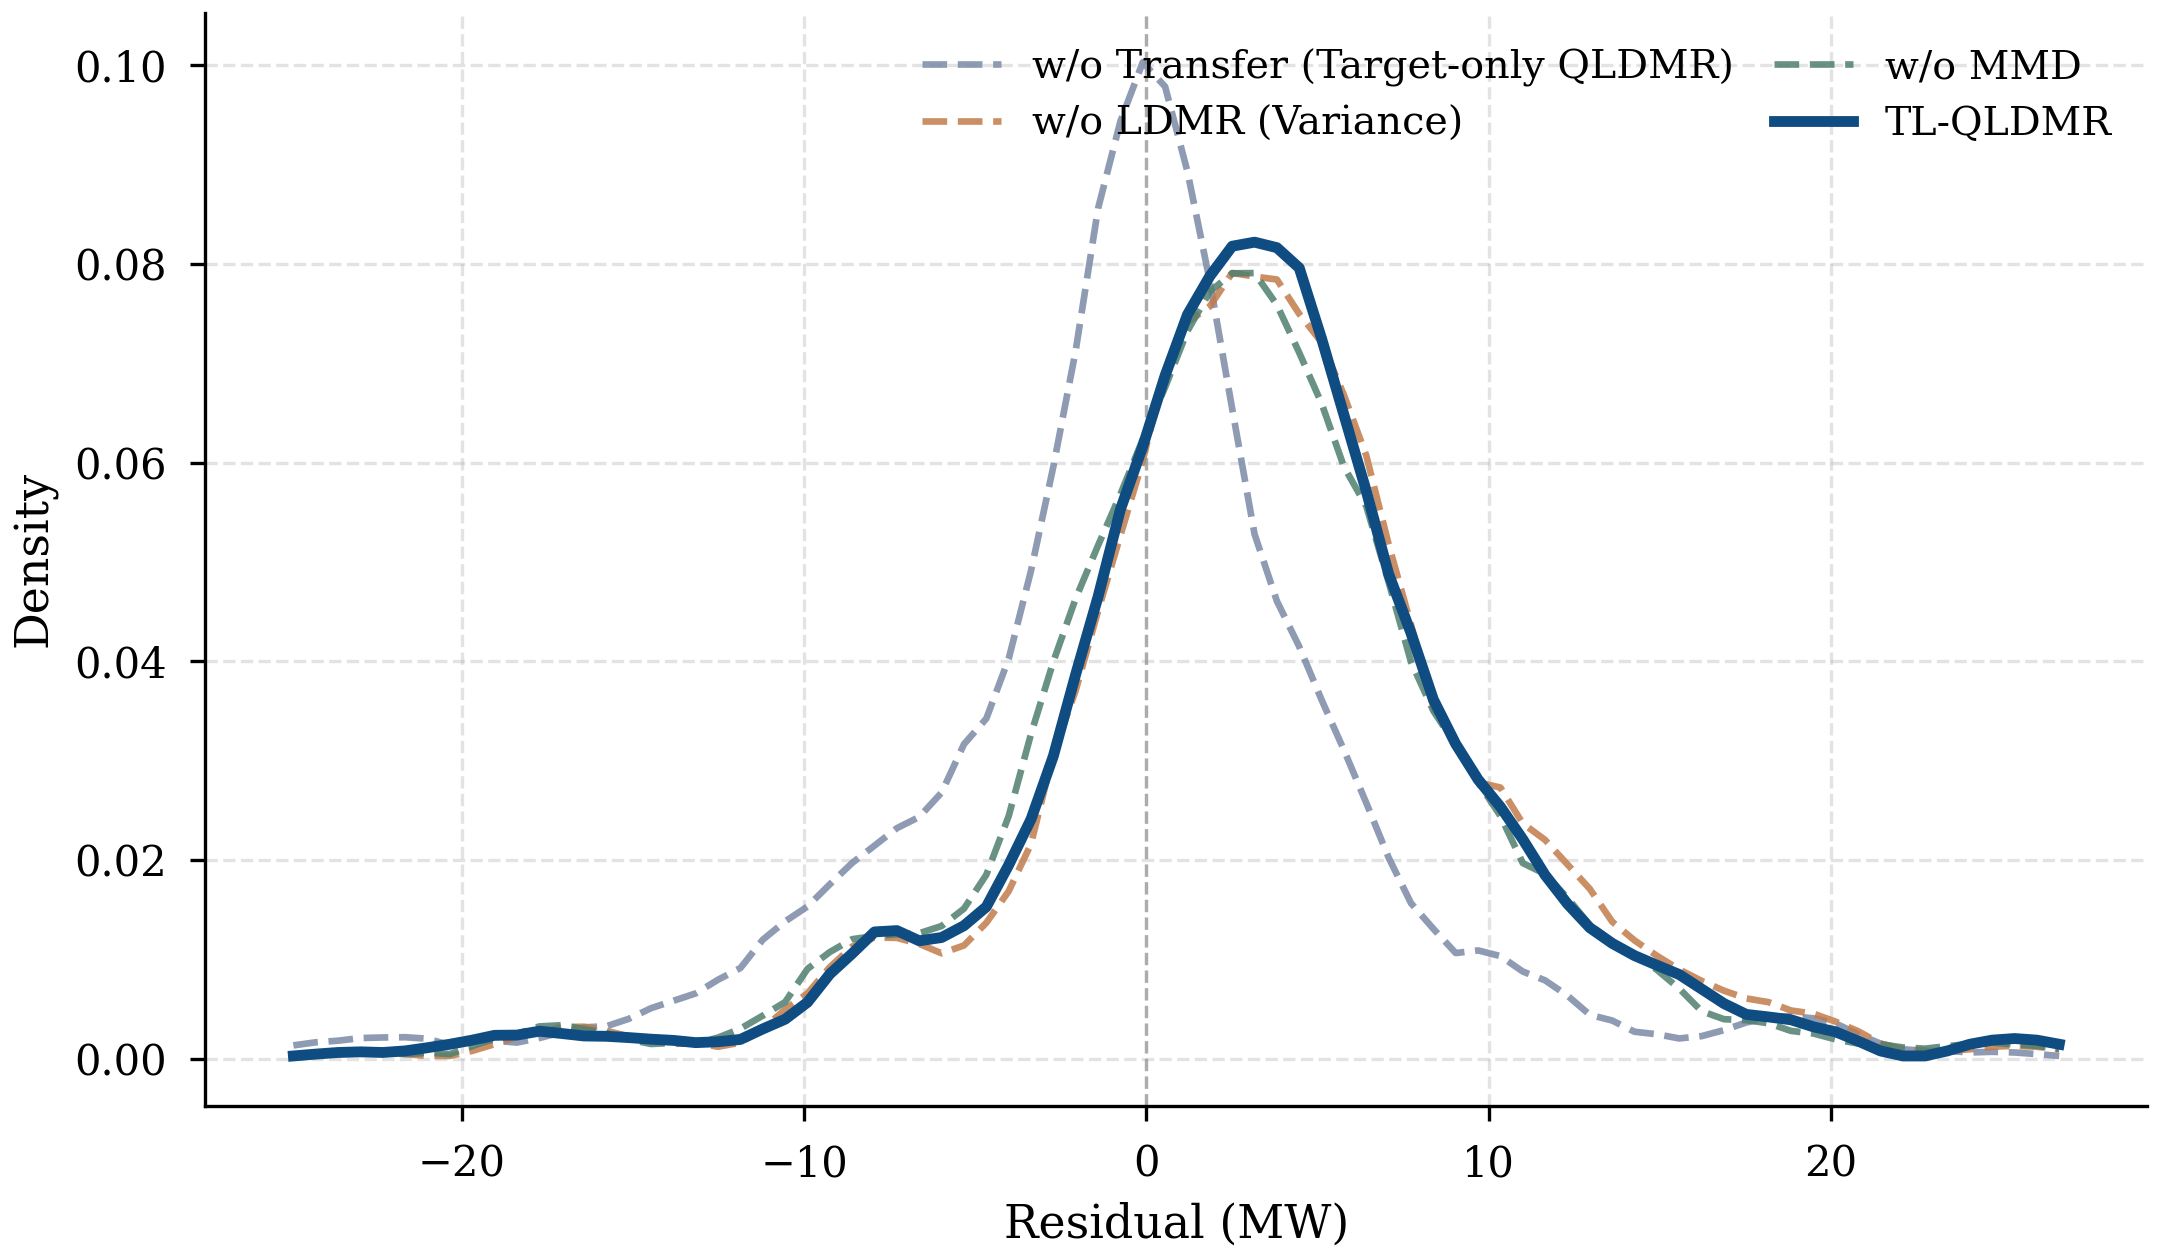
\includegraphics[width=0.82\linewidth]{experiment4/plots/residual_distribution.png}
\captionof{figure}{Residual density comparison between TL-QLDMR and ablated variants on the Farm~6 test set.}
\label{fig:ablation_residual}
\end{center}

The ablation outcomes confirm that each component contributes materially to robustness. Removing transfer learning reduces both point accuracy ($R^2$: 0.9557 $\rightarrow$ 0.9497) and interval quality (CWC: 0.2683 $\rightarrow$ 0.2797), indicating that target-only training is insufficient under strong domain shift. Removing LDMR regularization or MMD alignment causes clear interval-quality degradation (CWC rises to 0.3507 and 0.3528), even when point-metric changes are smaller, showing that residual-shape control and feature alignment are central to reliable uncertainty estimation.

Critically, the LDMR-Quantile (SymVar) variant, which replaces asymmetric variance with symmetric variance minimization, exhibits degraded performance on both point prediction (RMSE: 7.868 vs. 7.476) and interval prediction (CWC: 0.3029 vs. 0.2683, PINAW: 0.3029 vs. 0.2683). This degradation empirically validates our theoretical analysis in Section~\ref{novel}: symmetric variance minimization, while effective for mean regression, conflicts with the asymmetric residual distribution required for accurate quantile estimation. The symmetric regularizer forces errors toward a centered, Gaussian-like distribution, thereby degrading interval calibration at non-median quantiles.

The residual-density comparison in Fig.~\ref{fig:ablation_residual} supports this conclusion by showing tighter central concentration and weaker heavy tails for the full TL-QLDMR model; some ablated variants exhibit sharper central peaks but noticeably thicker tails, which corresponds to a higher probability of large-error events.
\FloatBarrier


%---------------- Experiment 5 --------------------%
\subsection{Experiment 5: Scalable Optimization Validation}\label{sec:exp5}

Experiment~5 evaluates whether the proposed Nystr\"{o}m-SGD solver can maintain computational efficiency as the training scale increases. The proposed solver is compared against three representative optimization baselines: (i) exact dual QP solved by the CVXOPT convex-optimization package, (ii) PyTorch-based gradient descent on the QP objective (Torch-GD), and (iii) mini-batch SGD with kernel-slice approximation.

To stress-test scalability, we consider seven training scales, increasing the combined training size from 100 to the full $N=69{,}737$. The evaluated sizes are $N=100, 500, 1{,}000, 3{,}000, 10{,}000, 30{,}000$, and $69{,}737$.
For each configuration, wall-clock training time (seconds) is recorded. Table~\ref{tab:scalability_results} summarizes the results.

\begin{table}[ht]
\centering
\caption{Training time (seconds) of four solvers over expanding training scales on Farm~6. ``---'' denotes runs not extended further because of prohibitive computational cost.}
{\small
\setlength{\tabcolsep}{2.6mm}
\begin{tabular}{rcccc}
\toprule
$N$ & CVXOPT & Torch-GD & Batch SGD & Nystr\"{o}m-SGD (Ours) \\
\midrule
100      & 0.509 & 2.155 & 2.746 & \textbf{0.035} \\
500      & 1.052 & 2.618 & 4.637 & \textbf{1.035} \\
1{,}000  & 7.655 & 2.979 & 5.699 & \textbf{1.038} \\
3{,}000  & --- & 20.395 & 6.418 & \textbf{2.468} \\
10{,}000 & --- & --- & 10.401 & \textbf{2.703} \\
30{,}000 & --- & --- & 25.338 & \textbf{3.483} \\
69{,}737 & --- & --- & --- & \textbf{5.021} \\
\bottomrule
\end{tabular}
}
\label{tab:scalability_results}
\end{table}

The full-QP routes lose practicality quickly as the scale increases. CVXOPT grows from 0.509 seconds at $N=100$ to 7.655 seconds at $N=1{,}000$ and is not extended further thereafter. Torch-GD remains workable slightly longer, but already requires 20.395 seconds at $N=3{,}000$, indicating that direct optimization of the kernel QP becomes inefficient well before the full training regime is reached.

Batch SGD avoids exact QP solving but remains substantially slower than the proposed Nystr\"{o}m-SGD solver at medium and large scales; for example, at $N=30{,}000$ it requires 25.338 seconds, compared with 3.483 seconds for the Nystr\"{o}m-SGD route. By contrast, the proposed solver is the only optimization route that completes the entire uncapped training set, reaching $N=69{,}737$ in 5.021 seconds. This trend is consistent with the theoretical reduction from $O(N^3)$ to $O(T \cdot N \cdot m)$: runtime growth remains comparatively mild even after the target-domain sample count saturates and the additional data come almost entirely from the source domain.


\section{Conclusion}\label{conclusion}
This paper presents TL-QLDMR for wind power forecasting under extreme events, where target-domain samples are limited and distribution shift is pronounced. The method combines asymmetric variance regularization, MMD-based feature alignment, and weighted pinball loss within a unified transfer-learning quantile framework, with theoretical guarantees on positive definiteness and convergence.

Experimental results show that TL-QLDMR delivers consistent gains in both deterministic and interval forecasting on the most challenging target farm. For point prediction, it achieves the best RMSE (7.478) and $R^2$ (0.9557). For 95\% interval prediction, it attains PICP $=0.959$ together with the best CWC (0.268), indicating a favorable reliability-sharpness trade-off. Under injected noise, TL-QLDMR remains the strongest model across reported point and interval metrics. In addition, the Nystr\"{o}m-SGD solver provides practical scalability, completing the full uncapped training set ($N=69{,}737$) in 5.021 seconds, whereas CVXOPT, Torch-GD, and batch SGD do not remain computationally viable at the same scale.

Future work will focus on extending the framework to multi-site spatiotemporal coupling, adaptive online recalibration under non-stationary weather, and hybrid kernel-deep transfer formulations.

%------------------------ Credit ------------------------
\printcredits


%------------------------ Declaration ------------------------
\section*{Declaration of Competing Interest}
The authors declare that they have no known competing financial interests or personal relationships that could have appeared to influence the work reported in this paper.


%------------------------ Acknowledgments ------------------------
\section*{Acknowledgments}
This work was supported in part by the National Natural Science Foundation of China under Grant 72471109 and Grant 62106205.



%------------------------ Reference ------------------------

\bibliographystyle{model5-names}
\bibliography{ref.bib}

\end{document}
